% !TEX program = xelatex
% !TEX encoding = UTF-8 Unicode

\documentclass[14pt,a4paper,oneside]{extreport}

% ==========================================================
% 1. NGÔN NGỮ VÀ FONT
% ==========================================================

\usepackage{fontspec}
\usepackage{polyglossia}

\setmainlanguage{vietnamese}
\setotherlanguage{english}

\setmainfont{Times New Roman}
\setsansfont{Arial}
\setmonofont{Courier New}

% ==========================================================
% 2. ĐỊNH DẠNG TRANG
% ==========================================================

\usepackage{geometry}
\usepackage{setspace}
\usepackage{indentfirst}
\usepackage{fancyhdr}
\usepackage{titlesec}
\usepackage{enumitem}

\geometry{
    top=30mm,
    bottom=25mm,
    left=35mm,
    right=20mm,
    headheight=18pt,
    headsep=8mm,
    footskip=15mm
}

\onehalfspacing

\setlength{\parindent}{1.27cm}
\setlength{\parskip}{0pt}
\setlength{\emergencystretch}{3em}

% ==========================================================
% 3. HÌNH ẢNH
% ==========================================================

\usepackage{graphicx}
\usepackage{float}
\usepackage{caption}
\usepackage{subcaption}

\graphicspath{{figures/}}

\captionsetup{
    font=small,
    labelfont=bf,
    justification=centering,
    labelsep=colon
}

\captionsetup[figure]{
    position=below,
    skip=8pt
}

\captionsetup[table]{
    position=above,
    skip=6pt
}

% ==========================================================
% 4. BẢNG
% ==========================================================

\usepackage{booktabs}
\usepackage{longtable}
\usepackage{array}
\usepackage{tabularx}
\usepackage{multirow}
\usepackage{makecell}

\renewcommand{\arraystretch}{1.25}

\newcolumntype{Y}{
    >{\raggedright\arraybackslash}X
}

\newcolumntype{L}[1]{
    >{\raggedright\arraybackslash}p{#1}
}

\newcolumntype{C}[1]{
    >{\centering\arraybackslash}p{#1}
}

\newcolumntype{R}[1]{
    >{\raggedleft\arraybackslash}p{#1}
}

% ==========================================================
% 5. TOÁN HỌC
% ==========================================================

\usepackage{amsmath}
\usepackage{amssymb}

% ==========================================================
% 6. DANH SÁCH
% ==========================================================

\setlist[itemize]{
    leftmargin=1.2cm,
    itemsep=2pt,
    topsep=4pt,
    parsep=0pt
}

\setlist[enumerate]{
    leftmargin=1.2cm,
    itemsep=2pt,
    topsep=4pt,
    parsep=0pt
}

% ==========================================================
% 7. ĐỊNH DẠNG CHƯƠNG VÀ MỤC
% ==========================================================

\titleformat{\chapter}[block]
    {\centering\Large\bfseries}
    {CHƯƠNG \thechapter.}
    {0.5em}
    {\MakeUppercase}

\titlespacing*{\chapter}
    {0pt}
    {-10pt}
    {20pt}

\titleformat{\section}
    {\large\bfseries}
    {\thesection}
    {0.8em}
    {}

\titleformat{\subsection}
    {\normalsize\bfseries}
    {\thesubsection}
    {0.8em}
    {}

\titleformat{\subsubsection}
    {\normalsize\bfseries\itshape}
    {\thesubsubsection}
    {0.8em}
    {}

\setcounter{secnumdepth}{3}
\setcounter{tocdepth}{3}

% ==========================================================
% 8. CODE LISTING
% ==========================================================

\usepackage{listings}
\usepackage{xcolor}

\definecolor{codegreen}{rgb}{0,0.55,0}
\definecolor{codegray}{rgb}{0.45,0.45,0.45}
\definecolor{codeblue}{rgb}{0,0,0.72}
\definecolor{codeorange}{rgb}{0.75,0.30,0}
\definecolor{backcolor}{rgb}{0.97,0.97,0.97}

\lstdefinestyle{mystyle}{
    backgroundcolor=\color{backcolor},
    commentstyle=\color{codegreen},
    keywordstyle=\color{codeblue}\bfseries,
    numberstyle=\tiny\color{codegray},
    stringstyle=\color{codeorange},
    basicstyle=\ttfamily\footnotesize,
    breakatwhitespace=false,
    breaklines=true,
    keepspaces=true,
    numbers=left,
    numbersep=7pt,
    showspaces=false,
    showstringspaces=false,
    showtabs=false,
    tabsize=4,
    frame=single,
    rulecolor=\color{codegray},
    captionpos=b
}

\lstset{style=mystyle}

% ==========================================================
% 9. HEADER VÀ FOOTER
% ==========================================================

\pagestyle{fancy}
\fancyhf{}

\fancyhead[L]{
    \small\textit{Đồ án môn Công nghệ Phần mềm}
}

\fancyhead[R]{
    \small\textit{AITasker Platform}
}

\fancyfoot[C]{
    \thepage
}

\renewcommand{\headrulewidth}{0.4pt}
\renewcommand{\footrulewidth}{0pt}

\fancypagestyle{plain}{
    \fancyhf{}
    \fancyfoot[C]{\thepage}
    \renewcommand{\headrulewidth}{0pt}
    \renewcommand{\footrulewidth}{0pt}
}

% ==========================================================
% 10. TÀI LIỆU THAM KHẢO
% ==========================================================

\usepackage{csquotes}

\usepackage[
    backend=biber,
    style=ieee,
    sorting=none,
    autolang=other
]{biblatex}

\DeclareLanguageMapping{vietnamese}{english}

\addbibresource{references.bib}

% ==========================================================
% 11. MỤC LỤC
% ==========================================================

\usepackage[nottoc]{tocbibind}

% ==========================================================
% 12. URL VÀ LIÊN KẾT PDF
% ==========================================================

\usepackage{xurl}
\usepackage{hyperref}
\usepackage{bookmark}

% Không đặt dòng trống bên trong khối hypersetup.
\hypersetup{
    unicode=true,
    colorlinks=true,
    linkcolor=black,
    citecolor=blue,
    urlcolor=blue,
    pdfauthor={Trương Tùng Hưng; Huỳnh Gia Văn; Nguyễn Minh Cường; Hoàng Quốc Khánh},
    pdftitle={AITasker - Nền tảng kết nối chuyên gia AI và doanh nghiệp cần tự động hóa bằng AI},
    pdfsubject={Báo cáo đồ án môn Công nghệ Phần mềm},
    pdfkeywords={AITasker, SRS, FastAPI, ReactJS, PostgreSQL, Artificial Intelligence},
    bookmarksopen=true,
    bookmarksnumbered=true
}

% ==========================================================
% 13. CÁC LỆNH TỰ ĐỊNH NGHĨA
% ==========================================================

\newcommand{\projectname}{AITasker}

\newcommand{\projectfullname}{
    Nền tảng kết nối chuyên gia AI và doanh nghiệp cần tự động hóa bằng AI
}

\newcommand{\universityname}{
    Trường Đại học Giao thông Vận tải Thành phố Hồ Chí Minh
}

\newcommand{\instructorname}{
    ThS. Nguyễn Văn Chiến
}

% ==========================================================
% BẮT ĐẦU TÀI LIỆU
% ==========================================================

\begin{document}

% Giảm cảnh báo tràn dòng đối với văn bản và URL dài.
\sloppy

% ==========================================================
% TRANG BÌA
% ==========================================================

\pagenumbering{gobble}

\begin{titlepage}

\begin{center}

%=========================================================
% BỘ GIÁO DỤC
%=========================================================

{\Large\textbf{BỘ GIÁO DỤC VÀ ĐÀO TẠO}}

\vspace{0.25cm}

{\Large\textbf{TRƯỜNG ĐẠI HỌC GIAO THÔNG VẬN TẢI}}

\vspace{0.1cm}

{\Large\textbf{THÀNH PHỐ HỒ CHÍ MINH}}

\vspace{0.25cm}

{\large\textbf{KHOA CÔNG NGHỆ THÔNG TIN}}

\vspace{0.1cm}

{\large\textbf{BỘ MÔN CÔNG NGHỆ PHẦN MỀM}}

\vspace{0.8cm}

%=========================================================
% LOGO
%=========================================================


\includegraphics[width=4.5cm]{figures/Logo_UTH.png}

\vspace{0.8cm}

%=========================================================
% TIÊU ĐỀ
%=========================================================

{\Large\textbf{ĐỒ ÁN MÔN HỌC}}

\vspace{0.35cm}

{\Huge\textbf{CÔNG NGHỆ PHẦN MỀM}}

\vspace{1.0cm}

\rule{0.9\textwidth}{1pt}

\vspace{0.8cm}

{\Huge\bfseries AITASKER}

\vspace{0.45cm}

{\Large\bfseries
NỀN TẢNG KẾT NỐI CHUYÊN GIA AI
}

\vspace{0.25cm}

{\Large\bfseries
VÀ DOANH NGHIỆP CẦN TỰ ĐỘNG HÓA BẰNG AI
}

\vspace{0.8cm}

\rule{0.9\textwidth}{0.6pt}

\vspace{1cm}

%=========================================================
% THÔNG TIN
%=========================================================

\renewcommand{\arraystretch}{1.5}

\begin{tabular}{p{5cm}p{9cm}}

\textbf{Giảng viên hướng dẫn:}
&
ThS. Nguyễn Văn Chiến
\\

\textbf{Môn học:}
&
Công nghệ Phần mềm
\\

\textbf{Nhóm thực hiện:}
&
Nhóm 07
\\

\textbf{Sinh viên:}
&
Trương Tùng Hưng
\\
&
Huỳnh Gia Văn
\\
&
Nguyễn Minh Cường
\\
&
Hoàng Quốc Khánh
\\

\textbf{MSSV:}
&
075206003322
\\
&
083206012872
\\
&
052206005225
\\
&
044205005486
\\

\textbf{Lớp:}
&
CNTTxxxx
\\

\textbf{Năm học:}
&
2025 -- 2026

\end{tabular}

\vfill

%=========================================================
% ĐỊA ĐIỂM
%=========================================================

{\large
TP. Hồ Chí Minh, tháng 07 năm 2026
}

\end{center}

\end{titlepage}

\clearpage

% ==========================================================
% PHẦN MỞ ĐẦU - SỐ TRANG LA MÃ
% ==========================================================

\pagenumbering{roman}
\setcounter{page}{1}

% ==========================================================
% LỜI CAM ĐOAN
% ==========================================================

\chapter*{Lời cam đoan}
\addcontentsline{toc}{chapter}{Lời cam đoan}

Chúng tôi cam đoan báo cáo đồ án môn học với đề tài
\textbf{``\projectname{} -- \projectfullname''}
là kết quả nghiên cứu và thực hiện của nhóm dưới sự hướng dẫn của
\instructorname.

Các nội dung phân tích, thiết kế, mã nguồn, số liệu và kết quả trình bày
trong báo cáo được nhóm thực hiện một cách trung thực. Những nội dung tham
khảo từ tài liệu, công trình nghiên cứu hoặc nguồn thông tin khác đều được
trích dẫn và ghi rõ nguồn trong phần tài liệu tham khảo.

Nhóm xin chịu trách nhiệm về tính trung thực và chính xác của nội dung
được trình bày trong báo cáo này.

\vspace{2.5cm}

\begin{flushright}
    \textit{TP. Hồ Chí Minh, tháng 07 năm 2026}\\[1cm]

    \textbf{Nhóm sinh viên thực hiện}\\[0.5cm]

    \textit{(Ký và ghi rõ họ tên)}
\end{flushright}

\clearpage

% ==========================================================
% LỜI CẢM ƠN
% ==========================================================

\chapter*{Lời cảm ơn}
\addcontentsline{toc}{chapter}{Lời cảm ơn}

Trước tiên, nhóm chúng tôi xin gửi lời cảm ơn chân thành đến
\instructorname, giảng viên hướng dẫn môn Công nghệ Phần mềm, đã tận tình
hướng dẫn, định hướng và đóng góp nhiều ý kiến quý báu trong suốt quá trình
thực hiện đồ án.

Nhóm xin chân thành cảm ơn quý thầy cô thuộc Khoa Công nghệ Thông tin,
\universityname{} đã truyền đạt những kiến thức nền tảng và chuyên ngành cần
thiết, đồng thời tạo điều kiện thuận lợi để nhóm có thể hoàn thành đề tài.

Trong quá trình thực hiện, mặc dù nhóm đã cố gắng nghiên cứu, phân tích và
hoàn thiện hệ thống, báo cáo vẫn khó tránh khỏi những thiếu sót. Nhóm rất mong
nhận được những ý kiến đóng góp từ quý thầy cô để hệ thống \projectname{} có
thể được tiếp tục hoàn thiện và phát triển trong tương lai.

\vspace{1cm}

\begin{flushright}
    \textbf{Nhóm sinh viên thực hiện}
\end{flushright}

\clearpage

% ==========================================================
% NHẬN XÉT CỦA GIẢNG VIÊN
% ==========================================================

\chapter*{Nhận xét của giảng viên hướng dẫn}
\addcontentsline{toc}{chapter}{Nhận xét của giảng viên hướng dẫn}

\vspace{0.5cm}

\noindent
\textbf{Nhận xét:}

\vspace{0.5cm}

\noindent
\rule{\textwidth}{0.4pt}\\[0.8cm]
\rule{\textwidth}{0.4pt}\\[0.8cm]
\rule{\textwidth}{0.4pt}\\[0.8cm]
\rule{\textwidth}{0.4pt}\\[0.8cm]
\rule{\textwidth}{0.4pt}\\[0.8cm]
\rule{\textwidth}{0.4pt}\\[0.8cm]
\rule{\textwidth}{0.4pt}\\[0.8cm]
\rule{\textwidth}{0.4pt}

\vfill

\begin{flushright}
    TP. Hồ Chí Minh, ngày \hspace{0.5cm}
    tháng \hspace{0.5cm} năm 2026\\[0.5cm]

    \textbf{Giảng viên hướng dẫn}\\[2cm]

    \textbf{\instructorname}
\end{flushright}

\clearpage

% ==========================================================
% MỤC LỤC
% ==========================================================

\tableofcontents

\clearpage

% ==========================================================
% DANH MỤC HÌNH ẢNH
% ==========================================================

\listoffigures

\clearpage

% ==========================================================
% DANH MỤC BẢNG
% ==========================================================

\listoftables

\clearpage

% ==========================================================
% DANH MỤC TỪ VIẾT TẮT
% ==========================================================

\chapter*{Danh mục từ viết tắt}
\addcontentsline{toc}{chapter}{Danh mục từ viết tắt}

\begin{longtable}{
    L{3cm}
    L{10.5cm}
}

\toprule
\textbf{Từ viết tắt}
&
\textbf{Ý nghĩa}
\\
\midrule
\endfirsthead

\toprule
\textbf{Từ viết tắt}
&
\textbf{Ý nghĩa}
\\
\midrule
\endhead

AI
&
Artificial Intelligence -- Trí tuệ nhân tạo.
\\

API
&
Application Programming Interface -- Giao diện lập trình ứng dụng.
\\

BCrypt
&
Thuật toán băm mật khẩu được sử dụng trong hệ thống.
\\

CI/CD
&
Continuous Integration/Continuous Delivery -- Tích hợp và triển khai liên tục.
\\

CNPM
&
Công nghệ Phần mềm.
\\

CSDL
&
Cơ sở dữ liệu.
\\

DB
&
Database -- Cơ sở dữ liệu.
\\

ERD
&
Entity Relationship Diagram -- Sơ đồ thực thể liên kết.
\\

FR
&
Functional Requirement -- Yêu cầu chức năng.
\\

HTTP
&
Hypertext Transfer Protocol.
\\

HTTPS
&
Hypertext Transfer Protocol Secure.
\\

JWT
&
JSON Web Token -- Chuẩn mã thông báo dùng để xác thực.
\\

NFR
&
Non-functional Requirement -- Yêu cầu phi chức năng.
\\

ORM
&
Object Relational Mapping -- Ánh xạ đối tượng quan hệ.
\\

RBAC
&
Role-Based Access Control -- Kiểm soát truy cập dựa trên vai trò.
\\

REST
&
Representational State Transfer.
\\

SRS
&
Software Requirements Specification -- Đặc tả yêu cầu phần mềm.
\\

UML
&
Unified Modeling Language -- Ngôn ngữ mô hình hóa thống nhất.
\\

UI
&
User Interface -- Giao diện người dùng.
\\

UX
&
User Experience -- Trải nghiệm người dùng.
\\

UUID
&
Universally Unique Identifier -- Mã định danh duy nhất toàn cục.
\\

\bottomrule

\end{longtable}

\clearpage

% ==========================================================
% NỘI DUNG CHÍNH - SỐ TRANG Ả RẬP
% ==========================================================

\pagenumbering{arabic}
\setcounter{page}{1}

% ==========================================================
% CÁC CHƯƠNG
% ==========================================================

\chapter{Giới thiệu đề tài}

\section{Đặt vấn đề}

Cuộc Cách mạng công nghiệp lần thứ tư cùng với sự phát triển nhanh chóng của trí tuệ nhân tạo (Artificial Intelligence - AI) đang tạo ra những thay đổi mạnh mẽ trong mọi lĩnh vực của đời sống kinh tế và xã hội. AI không còn chỉ là một công nghệ nghiên cứu mà đã trở thành công cụ quan trọng giúp doanh nghiệp nâng cao năng suất, tối ưu chi phí vận hành, tự động hóa quy trình nghiệp vụ và nâng cao khả năng cạnh tranh trên thị trường. Đặc biệt, sự xuất hiện của các mô hình AI tạo sinh (Generative AI) như ChatGPT, Gemini, Claude hay các mô hình mã nguồn mở đã giúp việc phát triển các giải pháp AI trở nên nhanh chóng, linh hoạt và dễ tiếp cận hơn bao giờ hết.
Tại Việt Nam cũng như trên thế giới, nhu cầu ứng dụng AI trong doanh nghiệp ngày càng gia tăng. Nhiều doanh nghiệp mong muốn triển khai các giải pháp như chatbot chăm sóc khách hàng, hệ thống phân tích dữ liệu, tự động hóa quy trình (AI Automation), xử lý tài liệu thông minh, trợ lý ảo, hệ thống đề xuất và các ứng dụng AI chuyên biệt khác nhằm nâng cao hiệu quả hoạt động và giảm chi phí nhân sự. Tuy nhiên, phần lớn doanh nghiệp, đặc biệt là các doanh nghiệp vừa và nhỏ, chưa sở hữu đội ngũ kỹ thuật có đủ chuyên môn để tự nghiên cứu và triển khai các hệ thống AI.
Bên cạnh đó, quá trình tìm kiếm đơn vị cung cấp dịch vụ AI hiện nay còn gặp nhiều khó khăn. Doanh nghiệp thường phải tìm kiếm thông qua các mối quan hệ cá nhân, mạng xã hội hoặc các nền tảng freelancer tổng quát. Những kênh này chưa được thiết kế riêng cho các dự án AI nên còn thiếu các cơ chế đánh giá chuyên môn, quản lý quy trình triển khai, theo dõi tiến độ và đảm bảo chất lượng dự án. Điều này làm tăng chi phí tìm kiếm đối tác, kéo dài thời gian triển khai và tiềm ẩn nhiều rủi ro trong quá trình hợp tác.
Ở chiều ngược lại, các chuyên gia AI, freelancer, startup công nghệ và các nhóm phát triển AI cũng gặp nhiều khó khăn trong việc tiếp cận khách hàng có nhu cầu thực sự. Mặc dù có năng lực chuyên môn cao, họ vẫn phải phụ thuộc vào các nền tảng việc làm chung hoặc hoạt động marketing cá nhân để tìm kiếm dự án. Điều này khiến việc xây dựng thương hiệu cá nhân, chứng minh năng lực và mở rộng thị trường trở nên khó khăn, đồng thời làm giảm cơ hội tiếp cận các dự án có giá trị lớn.
Ngoài ra, quá trình triển khai một dự án AI thường bao gồm nhiều giai đoạn như tiếp nhận yêu cầu, phân tích bài toán, báo giá, ký kết hợp đồng, trao đổi tài liệu, theo dõi tiến độ, nghiệm thu, thanh toán và đánh giá sau dự án. Hiện nay các bước này thường được quản lý thông qua nhiều công cụ riêng lẻ như email, Google Drive, Zalo, Slack hay các phần mềm quản lý công việc, dẫn đến dữ liệu bị phân tán, khó kiểm soát và làm giảm hiệu quả phối hợp giữa các bên.
Xuất phát từ những thực tiễn trên, nhóm nhận thấy cần có một nền tảng chuyên biệt dành riêng cho thị trường dịch vụ AI, đóng vai trò là cầu nối giữa doanh nghiệp và các chuyên gia AI. Nền tảng không chỉ giúp doanh nghiệp dễ dàng tìm kiếm đối tác phù hợp mà còn hỗ trợ các chuyên gia xây dựng hồ sơ năng lực, giới thiệu dịch vụ, nhận dự án và phát triển uy tín nghề nghiệp. Đồng thời, hệ thống cần tích hợp các chức năng quản lý toàn bộ vòng đời của dự án AI, bao gồm đăng yêu cầu, tìm kiếm chuyên gia, gửi đề xuất, trao đổi trực tuyến, quản lý tiến độ, thanh toán, đánh giá chất lượng và lưu trữ lịch sử hợp tác.
Từ những lý do trên, nhóm quyết định lựa chọn đề tài \textbf{AITasker – AI Marketplace Platform for AI Automation Services}. Hệ thống được định hướng xây dựng như một nền tảng Marketplace chuyên biệt dành cho lĩnh vực AI Automation, giúp kết nối hiệu quả giữa doanh nghiệp và các chuyên gia AI, nâng cao tính minh bạch trong quá trình hợp tác, tối ưu quy trình triển khai dự án và góp phần thúc đẩy quá trình chuyển đổi số trong doanh nghiệp. Đồng thời, đề tài cũng tạo điều kiện để nhóm vận dụng các kiến thức đã học về phát triển phần mềm, thiết kế hệ thống, cơ sở dữ liệu, điện toán đám mây và trí tuệ nhân tạo vào việc xây dựng một sản phẩm có tính ứng dụng thực tiễn cao.
\section{Lý do chọn đề tài}

Đề tài được lựa chọn dựa trên các lý do sau:

\begin{itemize}
    \item \textbf{Nhu cầu ứng dụng AI ngày càng gia tăng:} Trong bối cảnh chuyển đổi số diễn ra mạnh mẽ, trí tuệ nhân tạo (AI) đã trở thành một trong những công nghệ cốt lõi giúp doanh nghiệp nâng cao hiệu quả hoạt động. AI được ứng dụng trong nhiều lĩnh vực như chăm sóc khách hàng, phân tích dữ liệu, marketing, quản lý chuỗi cung ứng, sản xuất thông minh và tự động hóa quy trình nghiệp vụ. Việc ứng dụng AI không chỉ giúp tối ưu chi phí vận hành, giảm khối lượng công việc thủ công mà còn hỗ trợ doanh nghiệp đưa ra quyết định nhanh chóng và chính xác hơn, từ đó nâng cao năng lực cạnh tranh trên thị trường.
    \item \textbf{Thiếu nền tảng chuyên biệt cho dịch vụ AI:} Hiện nay, doanh nghiệp chủ yếu tìm kiếm chuyên gia AI thông qua các nền tảng freelancer tổng quát hoặc các kênh mạng xã hội. Tuy nhiên, những nền tảng này chưa được thiết kế riêng cho lĩnh vực AI nên thiếu các chức năng hỗ trợ đánh giá năng lực chuyên môn, quản lý dự án AI, báo giá và theo dõi tiến độ. Điều này khiến doanh nghiệp gặp nhiều khó khăn trong việc lựa chọn đối tác phù hợp, đồng thời các chuyên gia AI cũng khó tiếp cận đúng nhóm khách hàng có nhu cầu triển khai các giải pháp AI.
    \item \textbf{Xu hướng phát triển của AI và tự động hóa:} Sự phát triển nhanh chóng của các công nghệ như Machine Learning, Deep Learning, Generative AI, Large Language Models (LLMs) và AI Agents đang mở ra nhiều cơ hội để tự động hóa các quy trình nghiệp vụ trong doanh nghiệp. Các giải pháp AI Automation ngày càng được ứng dụng rộng rãi nhằm giảm chi phí, tăng năng suất và nâng cao chất lượng dịch vụ. Đây được xem là một trong những xu hướng công nghệ quan trọng, đóng vai trò thúc đẩy quá trình chuyển đổi số và phát triển kinh tế số trong tương lai.
    \item \textbf{Ý nghĩa thực tiễn của đề tài:} Việc xây dựng nền tảng \textbf{AITasker} góp phần giải quyết khoảng cách giữa doanh nghiệp có nhu cầu ứng dụng AI và các chuyên gia cung cấp dịch vụ AI. Hệ thống hỗ trợ doanh nghiệp dễ dàng đăng tải yêu cầu, tìm kiếm chuyên gia phù hợp, trao đổi thông tin, nhận báo giá, theo dõi tiến độ thực hiện và thanh toán trực tuyến. Đồng thời, nền tảng tạo môi trường minh bạch để các chuyên gia AI xây dựng hồ sơ năng lực, phát triển uy tín cá nhân và mở rộng cơ hội tiếp cận các dự án chất lượng.
    \item \textbf{Khả năng áp dụng kiến thức chuyên môn:} Đề tài là cơ hội để vận dụng tổng hợp các kiến thức đã học trong lĩnh vực Công nghệ thông tin như phân tích và thiết kế hệ thống, phát triển ứng dụng Web, lập trình Backend, thiết kế cơ sở dữ liệu, bảo mật hệ thống, điện toán đám mây, DevOps, API và tích hợp các dịch vụ AI hiện đại. Quá trình thực hiện đề tài giúp nhóm tích lũy kinh nghiệm xây dựng một hệ thống phần mềm hoàn chỉnh, có khả năng mở rộng, đáp ứng nhu cầu thực tế và phù hợp với xu hướng phát triển của ngành công nghệ.
\end{itemize}

\section{Mục tiêu đề tài}

Mục tiêu tổng quát của đề tài là xây dựng nền tảng \textbf{AITasker – AI Marketplace Platform for AI Automation Services}, đóng vai trò là cầu nối giữa doanh nghiệp có nhu cầu triển khai các giải pháp AI và các chuyên gia AI, freelancer hoặc nhóm phát triển. Hệ thống hướng đến việc hỗ trợ doanh nghiệp tìm kiếm chuyên gia phù hợp, quản lý toàn bộ quy trình thực hiện dự án và nâng cao hiệu quả hợp tác giữa các bên.
Để đạt được mục tiêu trên, đề tài đặt ra các mục tiêu cụ thể như sau:

\begin{itemize}
    \item Xây dựng nền tảng Marketplace chuyên biệt kết nối doanh nghiệp có nhu cầu triển khai các giải pháp AI với các chuyên gia AI, freelancer và đơn vị cung cấp dịch vụ AI, góp phần đơn giản hóa quá trình tìm kiếm và hợp tác giữa các bên.
    \item Xây dựng hệ thống quản lý tài khoản, xác thực người dùng và phân quyền theo từng vai trò (Doanh nghiệp, Chuyên gia AI và Quản trị viên), đảm bảo an toàn thông tin và kiểm soát quyền truy cập phù hợp với từng chức năng của hệ thống.
    \item Phát triển chức năng cho phép doanh nghiệp đăng tải yêu cầu hoặc dự án AI với đầy đủ thông tin như mô tả bài toán, mục tiêu, yêu cầu kỹ thuật, ngân sách, thời gian thực hiện và các tiêu chí lựa chọn chuyên gia.
    \item Xây dựng chức năng tìm kiếm, lọc và gợi ý các dự án phù hợp cho chuyên gia AI dựa trên lĩnh vực chuyên môn, kỹ năng, kinh nghiệm và lịch sử hoạt động, giúp nâng cao khả năng kết nối giữa doanh nghiệp và chuyên gia.
    \item Phát triển cơ chế gửi đề xuất thực hiện dự án (Proposal), báo giá, trao đổi thông tin và thương lượng giữa doanh nghiệp và chuyên gia trước khi ký kết hợp tác, tạo môi trường làm việc minh bạch và thuận tiện.
    \item Xây dựng hệ thống quản lý vòng đời dự án, hỗ trợ theo dõi tiến độ thực hiện, cập nhật trạng thái công việc, quản lý các mốc (Milestone), lưu trữ tài liệu và lịch sử trao đổi giữa các bên trong suốt quá trình triển khai.
    \item Xây dựng chức năng đánh giá, phản hồi và xếp hạng sau khi dự án hoàn thành nhằm tạo dựng uy tín cho doanh nghiệp và chuyên gia, đồng thời nâng cao chất lượng dịch vụ trên nền tảng.
    \item Nghiên cứu và tích hợp các kỹ thuật AI để hỗ trợ gợi ý chuyên gia phù hợp với yêu cầu dự án, đề xuất các dự án phù hợp với chuyên gia dựa trên hồ sơ năng lực, kỹ năng và lịch sử hợp tác, góp phần nâng cao hiệu quả kết nối.
    \item Thiết kế và triển khai hệ thống theo kiến trúc hiện đại, có khả năng mở rộng, đảm bảo tính bảo mật, hiệu năng, tính sẵn sàng và khả năng đáp ứng khi số lượng người dùng và dự án tăng lên trong tương lai.
\end{itemize}
\section{Đối tượng và phạm vi nghiên cứu}

\subsection{Đối tượng nghiên cứu}

Đề tài tập trung nghiên cứu các nội dung liên quan đến nền tảng Marketplace cung cấp dịch vụ AI, bao gồm mô hình kết nối giữa doanh nghiệp và chuyên gia AI, quy trình quản lý dự án, cơ chế trao đổi và cộng tác trực tuyến, cùng với các kỹ thuật gợi ý dựa trên AI để nâng cao hiệu quả kết nối.
Ngoài ra, đề tài cũng nghiên cứu các công nghệ phát triển ứng dụng Web hiện đại, hệ quản trị cơ sở dữ liệu, xác thực người dùng, bảo mật hệ thống và các giải pháp triển khai Backend phục vụ cho việc xây dựng một hệ thống hoàn chỉnh.

\subsection{Phạm vi nghiên cứu}

Đối tượng sử dụng hệ thống gồm:

\begin{itemize}
    \item \textbf{Doanh nghiệp:} Đăng tải dự án AI, tìm kiếm chuyên gia, trao đổi, quản lý tiến độ và đánh giá kết quả.
    \item \textbf{Chuyên gia AI/Freelancer:} Quản lý hồ sơ cá nhân, tìm kiếm dự án, gửi báo giá, trao đổi với khách hàng và thực hiện dự án.
    \item \textbf{Quản trị viên:} Quản lý người dùng, dự án, danh mục dịch vụ, xử lý báo cáo và giám sát hoạt động của hệ thống.
\end{itemize}

Trong phạm vi đề tài, hệ thống tập trung phát triển các chức năng chính sau:

\begin{itemize}
    \item Đăng ký, đăng nhập và xác thực người dùng.
    \item Quản lý hồ sơ cá nhân và hồ sơ năng lực.
    \item Đăng tải, chỉnh sửa và quản lý dự án AI.
    \item Tìm kiếm dự án và chuyên gia theo nhiều tiêu chí.
    \item Gửi, tiếp nhận và quản lý báo giá (Proposal).
    \item Chat và trao đổi trực tuyến giữa doanh nghiệp và chuyên gia.
    \item Theo dõi tiến độ thực hiện dự án.
    \item Đánh giá, nhận xét và xếp hạng sau khi hoàn thành dự án.
    \item Quản lý thông báo và lịch sử hoạt động.
    \item Chức năng quản trị hệ thống.
    \item Gợi ý chuyên gia hoặc dự án bằng AI.
\end{itemize}

Trong khuôn khổ đề tài, hệ thống tập trung xây dựng phiên bản Web phục vụ mục đích nghiên cứu và minh họa quy trình nghiệp vụ. Các chức năng thanh toán trực tuyến, ký hợp đồng điện tử hoặc triển khai ứng dụng di động sẽ được xem là hướng phát triển trong tương lai.

\section{Cấu trúc báo cáo}

Báo cáo được tổ chức thành sáu chương với nội dung chính như sau:

\begin{itemize}
    \item \textbf{Chương 1: Giới thiệu đề tài}
    Trình bày bối cảnh nghiên cứu, đặt vấn đề, lý do lựa chọn đề tài, mục tiêu nghiên cứu, đối tượng và phạm vi nghiên cứu, phương pháp thực hiện cũng như cấu trúc của báo cáo.

    \item \textbf{Chương 2: Khảo sát và phân tích yêu cầu hệ thống}
    Khảo sát thực trạng, phân tích bài toán, xác định các đối tượng sử dụng, xây dựng yêu cầu chức năng, yêu cầu phi chức năng và mô hình nghiệp vụ của hệ thống.

    \item \textbf{Chương 3: Phân tích và thiết kế hệ thống}
    Trình bày kiến trúc tổng thể của hệ thống, thiết kế cơ sở dữ liệu, xây dựng các sơ đồ UML như Use Case Diagram, Activity Diagram, Sequence Diagram, Class Diagram và thiết kế giao diện.

    \item \textbf{Chương 4: Xây dựng hệ thống}
    Giới thiệu các công nghệ được sử dụng, quá trình triển khai Backend, Frontend, cơ sở dữ liệu, API và xây dựng các chức năng chính của hệ thống.

    \item \textbf{Chương 5: Kiểm thử và đánh giá hệ thống}
    Thực hiện kiểm thử các chức năng của hệ thống, đánh giá kết quả đạt được, phân tích ưu điểm, hạn chế và mức độ đáp ứng các yêu cầu đã đặt ra.

    \item \textbf{Chương 6: Kết luận và hướng phát triển}
    Tổng kết những kết quả đạt được của đề tài, đánh giá đóng góp của hệ thống và đề xuất các hướng nghiên cứu, phát triển trong tương lai nhằm nâng cao tính ứng dụng của nền tảng.
\end{itemize}
\chapter{PHÂN TÍCH YÊU CẦU HỆ THỐNG}

\section{Giới thiệu chương}

Chương này trình bày quá trình khảo sát, phân tích và đặc tả yêu cầu của hệ thống \textbf{AITasker – AI Marketplace Platform for AI Automation Services}. Đây là giai đoạn quan trọng trong quá trình phát triển phần mềm, giúp xác định rõ bài toán cần giải quyết, phạm vi của hệ thống, các yêu cầu nghiệp vụ cũng như các yêu cầu kỹ thuật làm cơ sở cho việc thiết kế và triển khai ở các chương tiếp theo.
Trước hết, chương tiến hành khảo sát thực trạng của thị trường dịch vụ AI, phân tích những khó khăn mà doanh nghiệp và các chuyên gia AI đang gặp phải trong quá trình tìm kiếm, kết nối và hợp tác triển khai các dự án AI. Trên cơ sở đó, hệ thống được đề xuất nhằm giải quyết các vấn đề còn tồn tại, đồng thời đáp ứng nhu cầu ngày càng tăng về ứng dụng AI trong doanh nghiệp.
Tiếp theo, chương xây dựng tài liệu đặc tả yêu cầu phần mềm (Software Requirement Specification -- SRS), bao gồm việc xác định các tác nhân tham gia hệ thống, mô tả chức năng của từng nhóm người dùng và phân tích các yêu cầu chức năng, yêu cầu phi chức năng cũng như các ràng buộc cần đáp ứng. Những nội dung này là nền tảng để đảm bảo hệ thống được xây dựng đúng với mục tiêu và đáp ứng các yêu cầu của người sử dụng.
Bên cạnh đó, chương sử dụng ngôn ngữ mô hình hóa UML để mô tả trực quan các nghiệp vụ và quy trình xử lý của hệ thống thông qua các biểu đồ như Use Case Diagram, Activity Diagram, Sequence Diagram và Class Diagram. Đồng thời, mô hình dữ liệu được xây dựng bằng Entity Relationship Diagram (ERD) nhằm xác định các thực thể, thuộc tính và mối quan hệ giữa chúng, phục vụ cho việc thiết kế cơ sở dữ liệu của hệ thống.
Thông qua quá trình phân tích và mô hình hóa, các chức năng cốt lõi của nền tảng như quản lý người dùng, quản lý dự án AI, quản lý đề xuất (Proposal), trao đổi giữa doanh nghiệp và chuyên gia, quản lý tiến độ dự án, đánh giá sau khi hoàn thành dự án và quản trị hệ thống được xác định một cách đầy đủ và rõ ràng. Đồng thời, chương cũng làm rõ luồng tương tác giữa các thành phần của hệ thống, góp phần đảm bảo tính nhất quán trong quá trình thiết kế và phát triển.
Kết quả của chương là bộ tài liệu phân tích và đặc tả yêu cầu hoàn chỉnh, đóng vai trò làm nền tảng cho việc thiết kế kiến trúc hệ thống, thiết kế cơ sở dữ liệu, xây dựng các thành phần phần mềm và triển khai nền tảng \textbf{AITasker} trong các chương tiếp theo.
\section{Mô tả bài toán}

\subsection{Bối cảnh}

Trong bối cảnh cuộc Cách mạng công nghiệp lần thứ tư (Industry 4.0) và quá trình chuyển đổi số đang diễn ra mạnh mẽ trên phạm vi toàn cầu, trí tuệ nhân tạo (Artificial Intelligence -- AI) đã trở thành một trong những công nghệ nền tảng thúc đẩy đổi mới sáng tạo và nâng cao năng lực cạnh tranh của doanh nghiệp. AI được ứng dụng rộng rãi trong nhiều lĩnh vực như chăm sóc khách hàng, thương mại điện tử, tài chính, y tế, giáo dục, sản xuất, logistics và quản trị doanh nghiệp nhằm tự động hóa quy trình, phân tích dữ liệu, tối ưu hoạt động và hỗ trợ ra quyết định.
Trong những năm gần đây, sự phát triển vượt bậc của các công nghệ như Machine Learning, Deep Learning, Natural Language Processing (NLP), Computer Vision, Generative AI và Large Language Models (LLMs) đã mở ra nhiều cơ hội mới trong việc xây dựng các giải pháp AI có tính ứng dụng cao. Các mô hình AI hiện đại không chỉ giúp doanh nghiệp xử lý dữ liệu với quy mô lớn mà còn có khả năng tạo nội dung, phân tích tài liệu, xây dựng chatbot thông minh, trợ lý ảo và tự động hóa nhiều quy trình nghiệp vụ. Nhờ đó, việc ứng dụng AI ngày càng trở nên phổ biến và có chi phí triển khai phù hợp hơn đối với cả doanh nghiệp lớn lẫn doanh nghiệp vừa và nhỏ.
Cùng với sự phát triển của công nghệ, nhu cầu triển khai các dự án AI trong doanh nghiệp cũng gia tăng nhanh chóng. Nhiều tổ chức mong muốn ứng dụng AI để nâng cao chất lượng dịch vụ, tối ưu quy trình vận hành, giảm chi phí nhân sự và tạo ra các sản phẩm, dịch vụ thông minh. Tuy nhiên, quá trình triển khai các giải pháp AI thường đòi hỏi nguồn nhân lực có trình độ chuyên môn cao về khoa học dữ liệu, phát triển phần mềm, điện toán đám mây, xử lý dữ liệu và các thuật toán học máy. Đây là thách thức lớn đối với nhiều doanh nghiệp khi nguồn nhân lực AI chất lượng cao còn hạn chế và chi phí xây dựng đội ngũ nội bộ tương đối lớn.
Bên cạnh đó, các chuyên gia AI, freelancer và các công ty cung cấp dịch vụ AI cũng gặp không ít khó khăn trong việc tiếp cận khách hàng có nhu cầu thực tế. Phần lớn việc tìm kiếm dự án hiện nay vẫn thông qua các nền tảng freelancer tổng quát hoặc các kênh mạng xã hội, vốn chưa được thiết kế chuyên biệt cho lĩnh vực AI. Điều này khiến quá trình kết nối giữa doanh nghiệp và chuyên gia thiếu tính minh bạch, khó đánh giá năng lực chuyên môn, đồng thời chưa hỗ trợ đầy đủ các nghiệp vụ như quản lý dự án, báo giá, theo dõi tiến độ hay đánh giá chất lượng sau khi hoàn thành dự án.
Xuất phát từ thực trạng trên, việc xây dựng một nền tảng Marketplace chuyên biệt dành cho các dịch vụ AI là nhu cầu cần thiết. Một hệ thống như vậy sẽ đóng vai trò là cầu nối giữa doanh nghiệp và các chuyên gia AI, hỗ trợ toàn bộ quá trình hợp tác từ đăng tải yêu cầu, tìm kiếm chuyên gia, gửi đề xuất (Proposal), trao đổi thông tin, quản lý tiến độ, thanh toán đến đánh giá sau dự án. Không chỉ góp phần nâng cao hiệu quả triển khai các dự án AI, nền tảng còn thúc đẩy quá trình chuyển đổi số của doanh nghiệp và tạo môi trường phát triển bền vững cho cộng đồng chuyên gia AI.
\subsection{Thực trạng}

Hiện nay, cùng với sự phát triển mạnh mẽ của trí tuệ nhân tạo, nhu cầu triển khai các giải pháp AI trong doanh nghiệp ngày càng gia tăng. Tuy nhiên, thị trường cung cấp dịch vụ AI vẫn chưa có nhiều nền tảng chuyên biệt hỗ trợ kết nối hiệu quả giữa doanh nghiệp và các chuyên gia AI. Phần lớn doanh nghiệp hiện nay vẫn tìm kiếm đối tác thông qua các nền tảng tuyển dụng, marketplace freelancer hoặc các mạng xã hội nghề nghiệp. Mặc dù những kênh này sở hữu cộng đồng người dùng lớn, chúng chủ yếu phục vụ nhiều lĩnh vực khác nhau và chưa được thiết kế để đáp ứng các đặc thù của các dự án AI.
Đối với doanh nghiệp, việc tìm kiếm một chuyên gia hoặc đơn vị cung cấp dịch vụ AI phù hợp thường gặp nhiều khó khăn. Do đặc thù của lĩnh vực AI đòi hỏi kiến thức chuyên môn sâu về Machine Learning, Deep Learning, xử lý dữ liệu, phát triển mô hình và triển khai hệ thống, việc đánh giá năng lực của ứng viên thông qua hồ sơ hoặc thông tin giới thiệu là chưa đủ. Nhiều doanh nghiệp thiếu tiêu chí và công cụ để đánh giá chính xác kinh nghiệm thực tế, khả năng triển khai dự án cũng như chất lượng sản phẩm của các chuyên gia.
Ở chiều ngược lại, các chuyên gia AI, freelancer và các nhóm phát triển giải pháp AI cũng gặp khó khăn trong việc tiếp cận các doanh nghiệp có nhu cầu thực sự. Họ thường phải phụ thuộc vào các nền tảng freelancer tổng quát hoặc tự xây dựng thương hiệu cá nhân thông qua các kênh truyền thông. Điều này làm giảm khả năng tiếp cận các dự án phù hợp, đồng thời khiến quá trình xây dựng uy tín và mở rộng thị trường trở nên khó khăn hơn.
Bên cạnh đó, quá trình triển khai một dự án AI thường bao gồm nhiều giai đoạn như tiếp nhận yêu cầu, phân tích bài toán, gửi đề xuất (Proposal), thương lượng, quản lý tiến độ, nghiệm thu, thanh toán và đánh giá sau dự án. Trong thực tế, các hoạt động này thường được thực hiện thông qua nhiều công cụ riêng biệt như email, ứng dụng nhắn tin, lưu trữ đám mây hoặc các phần mềm quản lý công việc, dẫn đến dữ liệu bị phân tán, khó kiểm soát và thiếu tính đồng bộ trong quá trình hợp tác.
Một số hạn chế nổi bật của các nền tảng hiện nay có thể được tổng hợp như sau:

\begin{itemize}
    \item Khó đánh giá chính xác năng lực chuyên môn, kinh nghiệm triển khai và chất lượng công việc của các chuyên gia AI.
    \item Quá trình tìm kiếm, sàng lọc và lựa chọn chuyên gia phù hợp còn mất nhiều thời gian, chi phí và phụ thuộc nhiều vào đánh giá thủ công.
    \item Thiếu nền tảng chuyên biệt hỗ trợ doanh nghiệp và chuyên gia AI trao đổi yêu cầu kỹ thuật, gửi báo giá (Proposal), thương lượng và quản lý hợp đồng.
    \item Chưa hỗ trợ quản lý xuyên suốt vòng đời dự án AI, bao gồm theo dõi tiến độ, quản lý các mốc công việc (Milestone), lưu trữ tài liệu, lịch sử trao đổi và quá trình nghiệm thu.
    \item Hệ thống đánh giá, xếp hạng và phản hồi sau dự án còn hạn chế, gây khó khăn trong việc xây dựng uy tín và mức độ tin cậy giữa các bên.
    \item Chưa khai thác hiệu quả các công nghệ AI để gợi ý chuyên gia phù hợp với yêu cầu của doanh nghiệp hoặc đề xuất các dự án phù hợp với hồ sơ năng lực, kỹ năng và kinh nghiệm của chuyên gia.
    \item Khả năng tích hợp các dịch vụ hỗ trợ như thanh toán trực tuyến, thông báo theo thời gian thực, quản lý tài liệu và báo cáo tiến độ còn chưa đồng bộ, làm giảm hiệu quả phối hợp trong quá trình triển khai dự án.
\end{itemize}

Ở chiều ngược lại, các chuyên gia AI, freelancer và các nhóm phát triển giải pháp AI cũng gặp nhiều khó khăn trong việc tiếp cận khách hàng có nhu cầu thực sự. Nhiều chuyên gia phải tìm kiếm dự án thông qua các kênh trung gian hoặc mạng xã hội, dẫn đến khả năng tiếp cận khách hàng còn hạn chế, khó xây dựng uy tín cá nhân và mất nhiều thời gian trong quá trình tìm kiếm cơ hội hợp tác.
Từ những hạn chế trên, có thể thấy việc xây dựng một nền tảng chuyên biệt dành cho các dịch vụ AI là cần thiết. Nền tảng sẽ giúp kết nối doanh nghiệp với chuyên gia AI một cách hiệu quả, đồng thời hỗ trợ quản lý toàn bộ quy trình hợp tác từ đăng dự án, gửi báo giá, trao đổi, theo dõi tiến độ đến đánh giá sau khi hoàn thành dự án.
\subsection{Giải pháp đề xuất}

Đề tài xây dựng hệ thống AIConnect nhằm kết nối doanh nghiệp với các chuyên gia AI. Hệ thống hỗ trợ doanh nghiệp đăng tải dự án, tìm kiếm chuyên gia, ký kết hợp đồng, quản lý tiến độ và thanh toán trực tuyến.

Đối với chuyên gia AI, hệ thống cho phép tạo hồ sơ năng lực, tìm kiếm dự án, gửi đề xuất hợp tác và trao đổi trực tiếp với doanh nghiệp. Ngoài ra, hệ thống còn tích hợp chức năng AI Matching nhằm đề xuất chuyên gia phù hợp dựa trên kỹ năng, kinh nghiệm và lịch sử dự án.

\section{Đặc tả yêu cầu phần mềm (SRS)}

\subsection{Mục tiêu hệ thống}

AIConnect được xây dựng nhằm tạo ra nền tảng trung gian giúp doanh nghiệp và chuyên gia AI kết nối với nhau một cách nhanh chóng, minh bạch và hiệu quả. Hệ thống hỗ trợ toàn bộ quy trình từ đăng dự án, tìm kiếm chuyên gia, gửi đề xuất, ký hợp đồng, quản lý tiến độ, thanh toán đến đánh giá sau khi hoàn thành dự án.

\subsection{Đối tượng sử dụng}

Hệ thống gồm ba nhóm người dùng chính:
\begin{itemize}
    \item \textbf{Doanh nghiệp (Enterprise):} Đơn vị có nhu cầu giải quyết các bài toán AI.
    \item \textbf{Chuyên gia AI (Expert):} Cá nhân hoặc nhóm có năng lực triển khai giải pháp AI.
    \item \textbf{Quản trị viên (Admin):} Đơn vị vận hành và kiểm duyệt nền tảng.
\end{itemize}

\subsection{Yêu cầu chức năng}

\begin{table}[H]
\centering
\caption{Danh sách yêu cầu chức năng hệ thống}
\label{tab:functional_requirements}
\renewcommand{\arraystretch}{1.2}
\begin{tabular}{|c|p{8cm}|p{4cm}|}
\hline
\textbf{Mã} & \textbf{Mô tả yêu cầu} & \textbf{Tác nhân}\\
\hline
FR01 & Đăng ký tài khoản & Tất cả tác nhân\\
\hline
FR02 & Đăng nhập hệ thống & Tất cả tác nhân\\
\hline
FR03 & Quản lý hồ sơ cá nhân & Tất cả tác nhân\\
\hline
FR04 & Đăng dự án AI & Doanh nghiệp\\
\hline
FR05 & Tìm kiếm chuyên gia & Doanh nghiệp\\
\hline
FR06 & AI Matching chuyên gia & Doanh nghiệp\\
\hline
FR07 & Tạo hồ sơ chuyên gia & Chuyên gia\\
\hline
FR08 & Gửi đề xuất dự án & Chuyên gia\\
\hline
FR09 & Thuê chuyên gia & Doanh nghiệp\\
\hline
FR10 & Quản lý hợp đồng & Doanh nghiệp, Chuyên gia\\
\hline
FR11 & Quản lý tiến độ & Doanh nghiệp, Chuyên gia\\
\hline
FR12 & Chat trực tuyến & Doanh nghiệp, Chuyên gia\\
\hline
FR13 & Thanh toán trực tuyến & Doanh nghiệp\\
\hline
FR14 & Đánh giá dự án & Doanh nghiệp, Chuyên gia\\
\hline
FR15 & Quản lý người dùng & Admin\\
\hline
FR16 & Quản lý nội dung và kiểm duyệt & Admin\\
\hline
FR17 & Thống kê hệ thống & Admin\\
\hline
\end{tabular}
\end{table}

\subsection{Yêu cầu phi chức năng}

\begin{table}[H]
\centering
\caption{Danh sách yêu cầu phi chức năng}
\label{tab:non_functional_requirements}
\renewcommand{\arraystretch}{1.2}
\begin{tabular}{|c|p{12cm}|}
\hline
\textbf{Mã} & \textbf{Mô tả chi tiết kỹ thuật}\\
\hline
NFR01 & Thời gian phản hồi hệ thống nhỏ hơn 2 giây với các tác vụ thông thường.\\
\hline
NFR02 & Hỗ trợ tối thiểu 500 người dùng truy cập đồng thời tại một thời điểm.\\
\hline
NFR03 & Toàn bộ hệ thống giao tiếp qua giao thức bảo mật HTTPS.\\
\hline
NFR04 & Cơ chế xác thực phân quyền sử dụng JWT (JSON Web Token).\\
\hline
NFR05 & Mật khẩu người dùng được mã hóa một chiều bằng thuật toán BCrypt.\\
\hline
NFR06 & Hệ thống hoạt động liên tục với độ sẵn sàng cao 24/7.\\
\hline
NFR07 & Kiến trúc có khả năng mở rộng theo chiều ngang (Horizontal Scaling).\\
\hline
NFR08 & Hỗ trợ triển khai linh hoạt trên các nền tảng điện toán đám mây (Cloud).\\
\hline
NFR09 & Giao diện thích ứng (Responsive UI), thân thiện với người dùng.\\
\hline
NFR10 & Độ sẵn sàng của dịch vụ cốt lõi đạt tối thiểu 99.5\%.\\
\hline
\end{tabular}
\end{table}

\section{Xác định tác nhân hệ thống}

\subsection{Doanh nghiệp (Enterprise)}
Tác nhân đại diện cho các tổ chức, công ty có nhu cầu tìm kiếm nguồn lực công nghệ bên ngoài:
\begin{itemize}
    \item Đăng ký, đăng nhập và cập nhật hồ sơ pháp lý doanh nghiệp.
    \item Đăng tải thông tin, mô tả bài toán và ngân sách dự án AI.
    \item Sàng lọc, tìm kiếm và nhận đề xuất từ các chuyên gia.
    \item Phê duyệt đề xuất, ký kết hợp đồng điện tử và quản lý tiến độ.
    \item Giải ngân, thanh toán cột mốc và thực hiện đánh giá chuyên gia.
\end{itemize}

\subsection{Chuyên gia AI (Expert)}

Tác nhân đại diện cho các kỹ sư AI, nhà khoa học dữ liệu (Data Scientist), kỹ sư Machine Learning, kỹ sư MLOps, chuyên gia tự động hóa AI, freelancer hoặc các nhóm phát triển giải pháp AI có nhu cầu tìm kiếm cơ hội hợp tác với doanh nghiệp. Đây là nhóm người dùng trực tiếp cung cấp các dịch vụ AI trên nền tảng.

\begin{itemize}
    \item Đăng ký, đăng nhập và quản lý thông tin tài khoản cá nhân.
    \item Xây dựng hồ sơ năng lực (Portfolio), cập nhật thông tin cá nhân, kỹ năng, chứng chỉ, kinh nghiệm làm việc, dự án đã thực hiện và các lĩnh vực chuyên môn.
    \item Thiết lập danh mục dịch vụ AI cung cấp và mức giá tham khảo.
    \item Tìm kiếm, lọc và theo dõi các dự án AI phù hợp với kỹ năng, kinh nghiệm và lĩnh vực chuyên môn.
    \item Gửi Proposal (đề xuất thực hiện dự án), báo giá, thời gian triển khai và kế hoạch thực hiện cho doanh nghiệp.
    \item Trao đổi trực tiếp với doanh nghiệp thông qua hệ thống nhắn tin để làm rõ yêu cầu, thương lượng ngân sách và phạm vi công việc.
    \item Tham gia triển khai dự án sau khi được doanh nghiệp lựa chọn.
    \item Cập nhật tiến độ thực hiện, quản lý các mốc công việc (Milestones), tải lên tài liệu, sản phẩm và báo cáo kết quả trong quá trình triển khai.
    \item Theo dõi trạng thái dự án, lịch sử hợp tác, các khoản thanh toán và doanh thu từ các dự án đã hoàn thành.
    \item Nhận thanh toán sau khi dự án hoặc từng mốc công việc được doanh nghiệp nghiệm thu.
    \item Đánh giá và phản hồi doanh nghiệp sau khi kết thúc dự án nhằm xây dựng môi trường hợp tác minh bạch và nâng cao chất lượng dịch vụ.
\end{itemize}

\subsection{Quản trị viên (Admin)}

Quản trị viên là tác nhân chịu trách nhiệm quản lý, vận hành và giám sát toàn bộ nền tảng nhằm đảm bảo hệ thống hoạt động ổn định, an toàn và minh bạch. Admin có quyền truy cập cao nhất và thực hiện các nghiệp vụ quản trị liên quan đến người dùng, dự án và hệ thống.

\begin{itemize}
    \item Quản lý toàn bộ tài khoản người dùng, bao gồm doanh nghiệp, chuyên gia AI và các tài khoản quản trị.
    \item Phê duyệt, khóa, mở khóa hoặc phân quyền tài khoản khi cần thiết.
    \item Kiểm duyệt các bài đăng dự án, hồ sơ chuyên gia và nội dung trên nền tảng nhằm đảm bảo tuân thủ các quy định và chính sách của hệ thống.
    \item Giám sát quá trình hợp tác giữa doanh nghiệp và chuyên gia, hỗ trợ xử lý các khiếu nại, tranh chấp hoặc vi phạm trong quá trình thực hiện dự án.
    \item Quản lý các giao dịch tài chính, theo dõi thanh toán, giải ngân và kiểm tra các giao dịch bất thường.
    \item Quản lý danh mục kỹ năng, lĩnh vực AI, danh mục dịch vụ và các dữ liệu dùng chung của hệ thống.
    \item Theo dõi tình trạng hoạt động của hệ thống, giám sát nhật ký (Log), hiệu năng và các cảnh báo bảo mật.
    \item Thống kê, tổng hợp và phân tích dữ liệu hoạt động của nền tảng thông qua các báo cáo về số lượng người dùng, dự án, doanh thu, giao dịch và các chỉ số tăng trưởng.
    \item Quản lý cấu hình hệ thống, gửi thông báo đến người dùng và hỗ trợ bảo trì, nâng cấp hệ thống khi cần thiết.
\end{itemize}

\section{Danh sách Use Case}

Mô hình Use Case tổng thể được bóc tách chi tiết thông qua các hành vi đặc trưng của từng tác nhân được liệt kê chi tiết trong Bảng \ref{tab:usecase}.

\begin{table}[H]
\centering
\caption{Danh sách Use Case của hệ thống AIConnect}
\label{tab:usecase}
\renewcommand{\arraystretch}{1.2}
\begin{tabular}{|c|p{8cm}|p{4cm}|}
\hline
\textbf{Mã} & \textbf{Tên Use Case} & \textbf{Tác nhân}\\
\hline
UC01 & Đăng ký tài khoản & Tất cả tác nhân\\
\hline
UC02 & Đăng nhập hệ thống & Tất cả tác nhân\\
\hline
UC03 & Quản lý hồ sơ cá nhân & Tất cả tác nhân\\
\hline
UC04 & Đăng dự án AI & Doanh nghiệp\\
\hline
UC05 & Tìm kiếm chuyên gia & Doanh nghiệp\\
\hline
UC06 & AI Matching chuyên gia & Doanh nghiệp\\
\hline
UC07 & Tạo hồ sơ chuyên gia & Chuyên gia\\
\hline
UC08 & Gửi đề xuất dự án & Chuyên gia\\
\hline
UC09 & Thuê chuyên gia & Doanh nghiệp\\
\hline
UC10 & Quản lý hợp đồng & Doanh nghiệp, Chuyên gia\\
\hline
UC11 & Quản lý tiến độ dự án & Doanh nghiệp, Chuyên gia\\
\hline
UC12 & Chat trực tuyến & Doanh nghiệp, Chuyên gia\\
\hline
UC13 & Thanh toán trực tuyến & Doanh nghiệp\\
\hline
UC14 & Đánh giá dự án & Doanh nghiệp, Chuyên gia\\
\hline
UC15 & Quản lý người dùng & Admin\\
\hline
UC16 & Kiểm duyệt nội dung & Admin\\
\hline
UC17 & Xem thống kê hệ thống & Admin\\
\hline
\end{tabular}
\end{table}

\section{Biểu đồ Use Case}

Biểu đồ Use Case mô tả trực quan các ranh giới chức năng chính của hệ thống và mối tương quan tương tác giữa các nhóm tác nhân với nền tảng.

\begin{figure}[H]
\centering
\includegraphics[width=0.3\textwidth]{figures/usecase.png}
\caption{Biểu đồ Use Case tổng thể hệ thống AIConnect}
\label{fig:usecase_diagram}
\end{figure}

Thông qua mô hình hóa Use Case, luồng chức năng phân hệ được phân định rõ ràng. Doanh nghiệp nắm giữ các quyền cốt lõi về mặt tài chính và điều phối công việc như đăng bài, chọn đối tác và thanh toán. Chuyên gia tập trung vào các hành vi thể hiện năng lực và phản hồi kết quả công việc. Trong khi đó, nhóm Admin vận hành độc lập ở phân hệ quản trị hệ thống.

\section{Biểu đồ Activity}

\subsection{Activity Diagram chức năng đăng nhập}
Biểu đồ hoạt động mô tả tiến trình xác thực danh tính người dùng khi truy cập vào hệ thống nền tảng.

\begin{figure}[H]
\centering
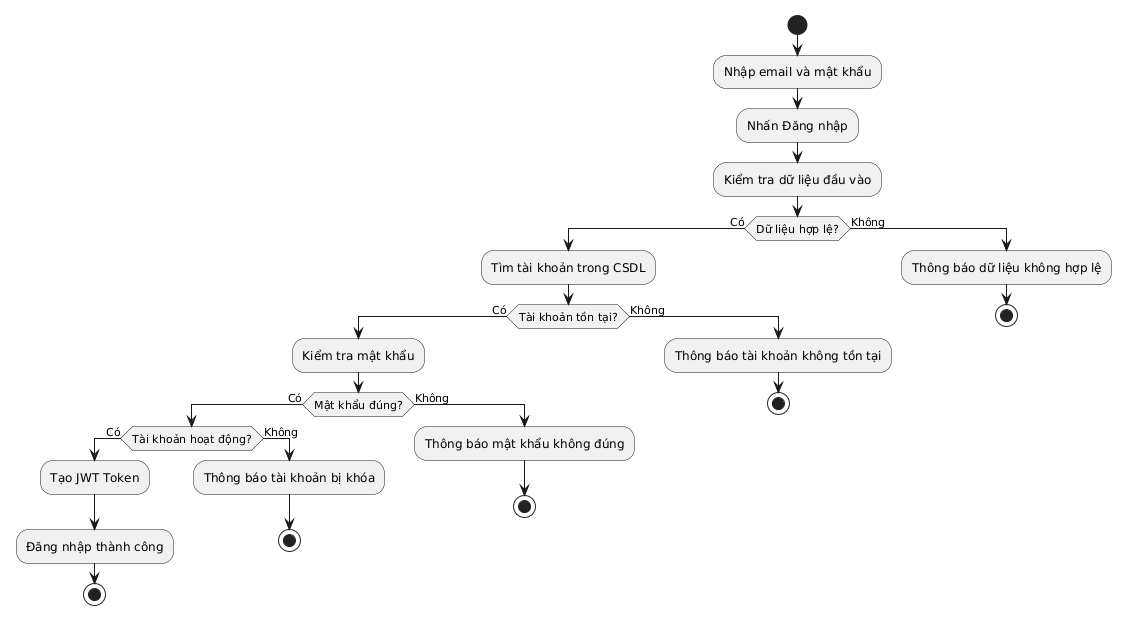
\includegraphics[width=0.7\textwidth]{figures/activity1.png}
\caption{Activity Diagram chức năng đăng nhập}
\label{fig:activity_login}
\end{figure}

Quy trình bắt đầu khi người dùng nhập thông tin định danh bao gồm Email và Mật khẩu. Hệ thống tiến hành truy vấn kiểm tra sự tồn tại của tài khoản trong cơ sở dữ liệu. Nếu tài khoản không tồn tại hoặc mật khẩu băm đối sánh (BCrypt) không trùng khớp, hệ thống sẽ trả về thông báo lỗi và yêu cầu nhập lại. Nếu thông tin hoàn toàn hợp lệ, hệ thống tiến hành cấp phát mã mã hóa JWT Token, chuyển hướng người dùng vào trang giao diện Dashboard tương ứng với vai trò của họ.

\subsection{Activity Diagram chức năng đăng tải dự án}
Biểu đồ mô tả luồng nghiệp vụ khi tác nhân Doanh nghiệp khởi tạo và công bố một bài toán công nghệ mới lên cộng đồng.

\begin{figure}[H]
\centering
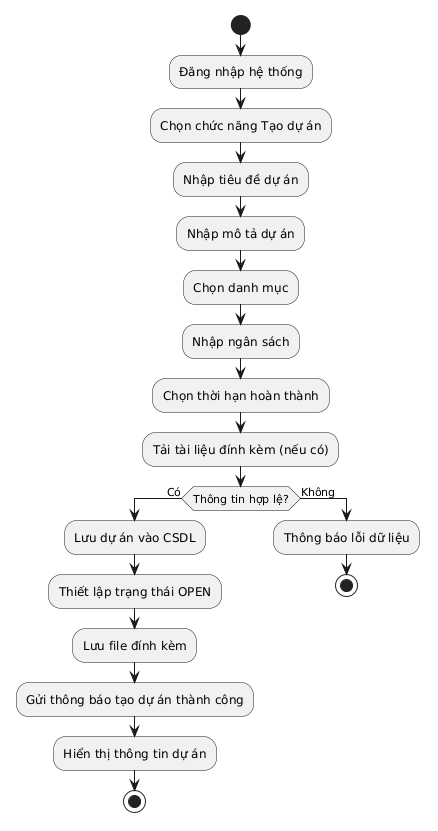
\includegraphics[width=0.45\textwidth]{figures/activity2.png}
\caption{Activity Diagram chức năng đăng tải dự án}
\label{fig:activity_create_project}
\end{figure}

Doanh nghiệp chọn tính năng đăng dự án và hoàn thiện biểu mẫu thông tin (Tiêu đề, mô tả bài toán, ngân sách, yêu cầu kỹ thuật và danh mục công nghệ). Hệ thống sẽ thực hiện kiểm tra tính hợp lệ của dữ liệu đầu vào. Tiếp theo, hệ thống rẽ nhánh kiểm tra sự tồn tại của tệp tài liệu đính kèm kèm theo. Nếu có, tệp tin sẽ được tải lên hệ thống lưu trữ và liên kết đường dẫn. Sau khi hoàn tất lưu bản ghi dự án với trạng thái \texttt{OPEN}, hệ thống kích hoạt Dịch vụ thông báo để lưu log đồng thời hiển thị thông báo thành công ra màn hình Client.

\subsection{Activity Diagram chức năng gửi đề xuất}
Biểu đồ hoạt động mô tả chi tiết quy trình nghiệp vụ và các bước kiểm tra logic khi chuyên gia AI chủ động nộp hồ sơ giải pháp cho dự án.

\begin{figure}[H]
\centering
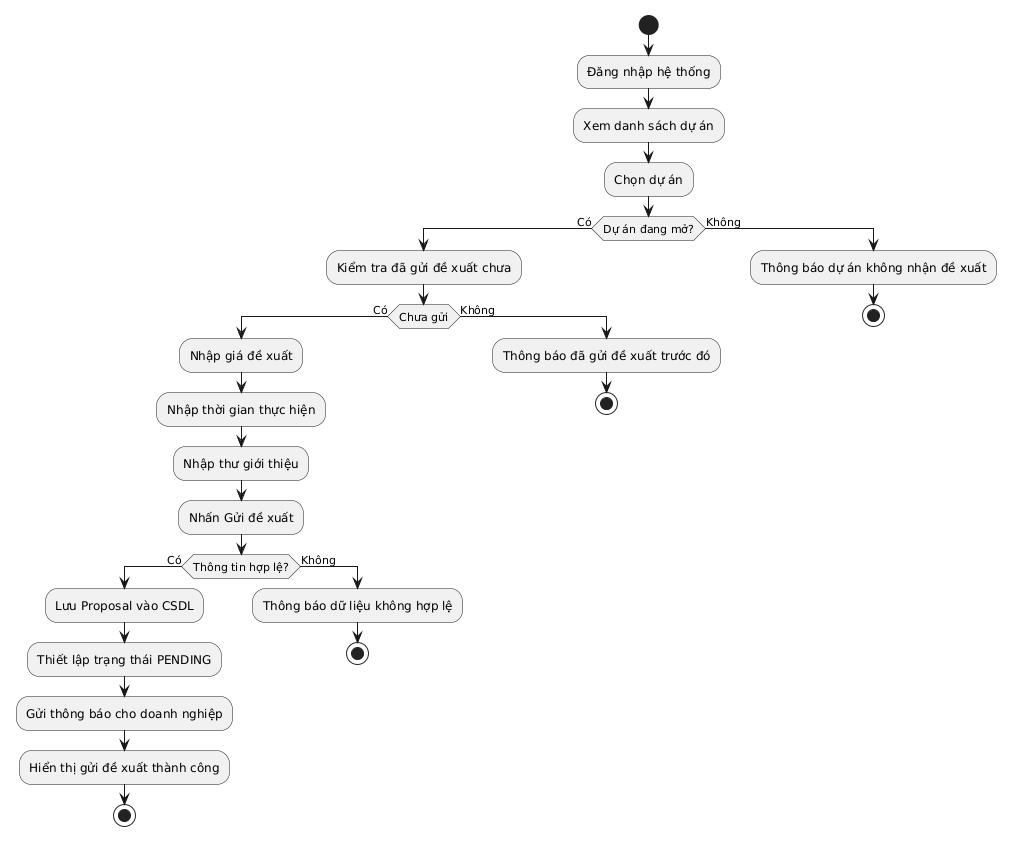
\includegraphics[width=0.7\textwidth]{figures/activity3.png}
\caption{Activity Diagram chức năng gửi đề xuất dự án}
\label{fig:activity_submit_proposal}
\end{figure}

Quy trình nghiệp vụ yêu cầu chuyên gia phải đăng nhập hợp lệ. Khi một dự án được chọn, hệ thống sẽ chạy tiến trình kiểm tra trạng thái song song: đảm bảo dự án vẫn trong thời hạn nhận hồ sơ và chuyên gia này chưa từng nộp đề xuất nào trước đó. Form nhập liệu yêu cầu đầy đủ các thông số tài chính và kỹ thuật trước khi lưu dữ liệu xuống phân hệ lưu trữ.

\subsection{Activity Diagram chức năng thuê chuyên gia}
Sơ đồ mô tả quy trình chuyển đổi trạng thái mang tính chất giao dịch khi doanh nghiệp chấp thuận một chuyên gia thực hiện dự án.

\begin{figure}[H]
\centering
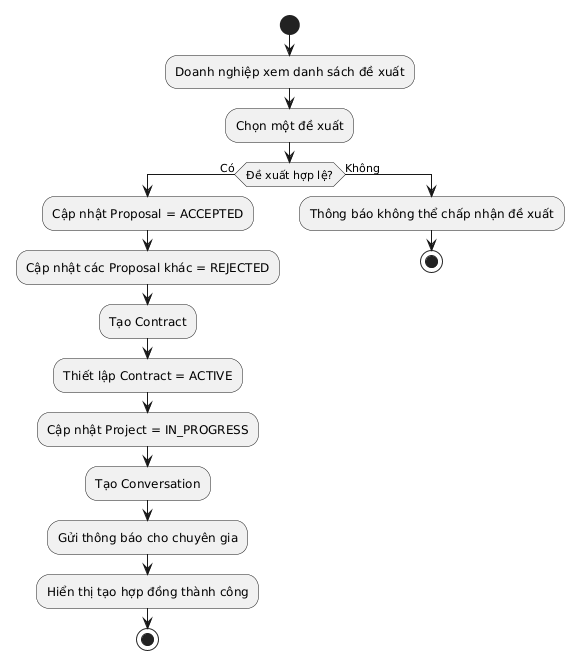
\includegraphics[width=0.7\textwidth]{figures/activity4.png}
\caption{Activity Diagram chức năng thuê chuyên gia và tạo hợp đồng}
\label{fig:activity_hire_expert}
\end{figure}

Tiến trình xử lý tự động hóa của hệ thống đảm bảo tính toàn vẹn: khi một đề xuất chuyển sang trạng thái \texttt{ACCEPTED}, toàn bộ các đề xuất ứng tuyển đồng cấp khác lập tức chuyển thành \texttt{REJECTED}. Các thực thể phụ thuộc như Hợp đồng mới và Kênh giao tiếp thời gian thực cũng đồng thời được khởi tạo trong cùng một phiên xử lý.

\subsection{Activity Diagram chức năng thanh toán}
Biểu đồ hoạt động mô tả quy trình giải ngân tài chính cho từng cột mốc công việc dựa trên việc kết nối với cổng thanh toán điện tử ngoại vi.

\begin{figure}[H]
\centering
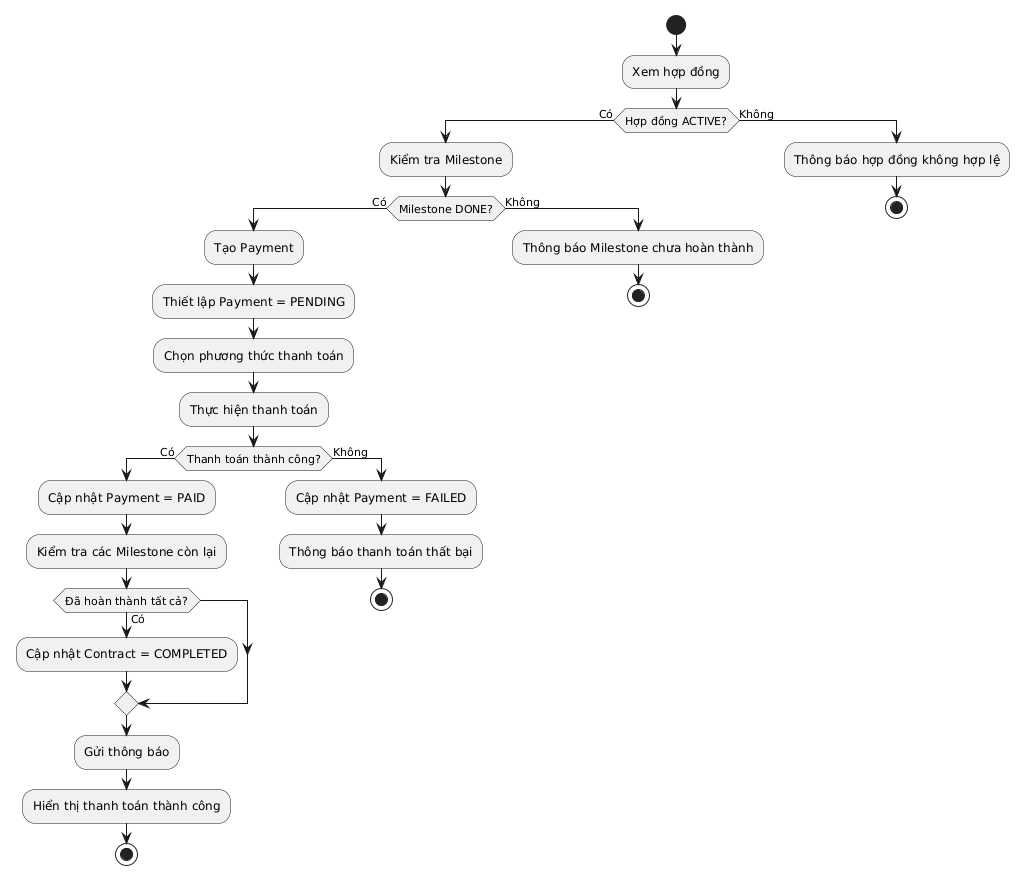
\includegraphics[width=0.7\textwidth]{figures/activity5.png}
\caption{Activity Diagram chức năng thanh toán giai đoạn}
\label{fig:activity_payment}
\end{figure}

Doanh nghiệp thực hiện kích hoạt lệnh giải ngân cho một cột mốc công việc đã được nghiệm thu kỹ thuật. Hệ thống kiểm tra điều kiện trạng thái của hợp đồng (\texttt{ACTIVE}) và trạng thái cột mốc (\texttt{DONE}). Nếu hợp lệ, một bản ghi giao dịch với trạng thái \texttt{PENDING} được thiết lập và hệ thống điều hướng người dùng sang giao diện của bên thứ ba (Cổng thanh toán). Tùy thuộc vào gói tin phản hồi trả về, hệ thống cập nhật kết quả thành \texttt{PAID} (Thành công) hoặc \texttt{FAILED} (Thất bại), ghi nhận vào nhật ký hệ thống và phát thông báo đến cả hai bên tác nhân.

\subsection{Activity Diagram chức năng đánh giá dự án}
Luồng hoạt động đóng vai trò chốt chặn cuối cùng nhằm cập nhật chỉ số uy tín của các bên sau khi hợp đồng kết thúc.

\begin{figure}[H]
\centering
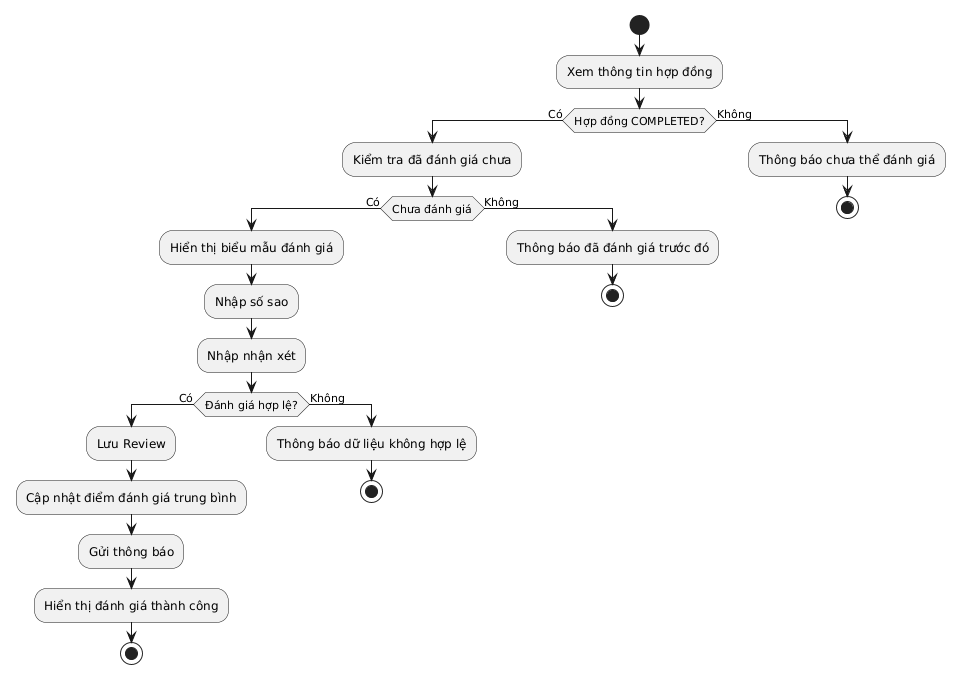
\includegraphics[width=0.7\textwidth]{figures/activity6.png}
\caption{Activity Diagram chức năng đánh giá kết quả dự án}
\label{fig:activity_review_project}
\end{figure}

Hệ thống chỉ kích hoạt quyền đánh giá khi kiểm tra bản ghi hợp đồng đã chuyển hẳn sang trạng thái \texttt{COMPLETED}. Điểm số sao (\texttt{rating}) sau khi được biểu mẫu thu thập sẽ được đưa vào hàm thuật toán tính toán lại điểm trung bình tích lũy trước khi cập nhật trực tiếp vào hồ sơ tổng của người dùng.

\section{Biểu đồ Sequence}

\subsection{Sequence Diagram chức năng đăng nhập}
Mô tả trình tự trao đổi thông điệp xác thực an toàn giữa Client và Server sử dụng cơ chế chữ ký điện tử JWT.

\begin{figure}[H]
\centering
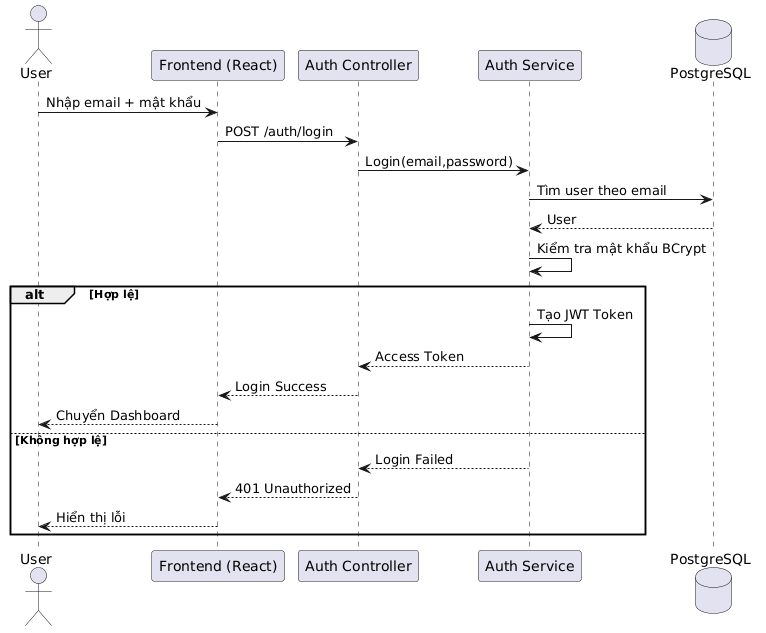
\includegraphics[width=\textwidth]{figures/sequence1.png}
\caption{Sequence Diagram chức năng đăng nhập hệ thống}
\label{fig:sequence_login}
\end{figure}

Mô hình tương tác thể hiện rõ lớp bảo mật tại tầng dịch vụ (\texttt{AuthService}). Tiến trình băm mật khẩu đối sánh được xử lý tuần tự trước khi tạo chuỗi mã hóa \texttt{AccessToken} để Frontend lưu trữ và điều hướng màn hình.

\subsection{Sequence Diagram chức năng đăng dự án}
Sơ đồ tuần tự thể hiện các bước nghiệp vụ tạo bài đăng công nghệ mới kết hợp lưu trữ tệp tin đính kèm.

\begin{figure}[H]
\centering
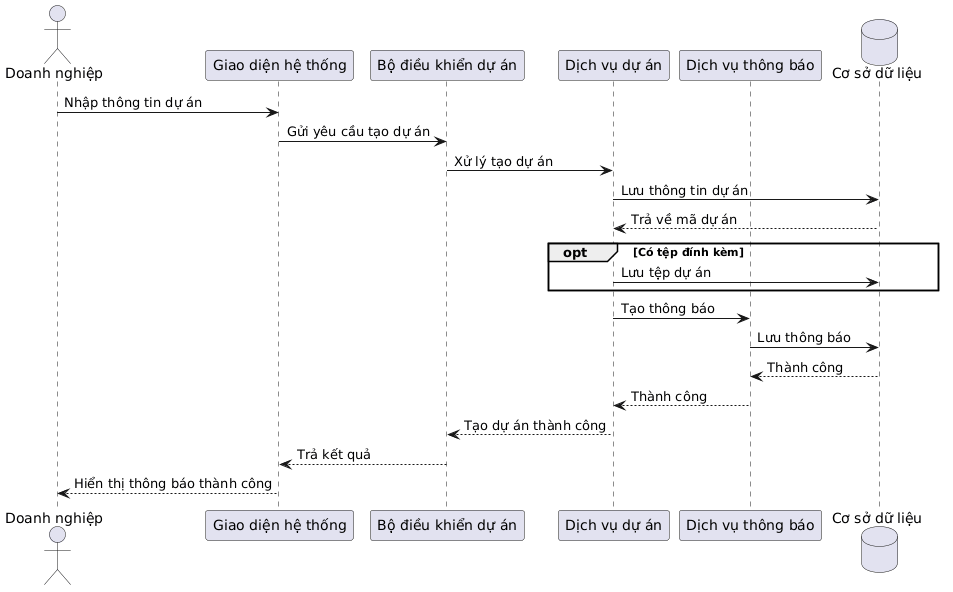
\includegraphics[width=\textwidth]{figures/sequence2.png}
\caption{Sequence Diagram chức năng đăng tải dự án}
\label{fig:sequence_create_project}
\end{figure}

Luồng xử lý bộc lộ tính kết hợp giữa lưu trữ dữ liệu cấu trúc (PostgreSQL) và xử lý tệp tin đa phương tiện. Khi \texttt{Project ID} được sinh ra, các tệp tài liệu đi kèm mới chính thức được ánh xạ và lưu vào hệ thống dữ liệu.

\subsection{Sequence Diagram chức năng gửi đề xuất}
Trình tự gọi hàm kiểm tra điều kiện ràng buộc nghiệp vụ khi chuyên gia gửi báo giá giải pháp.

\begin{figure}[H]
\centering
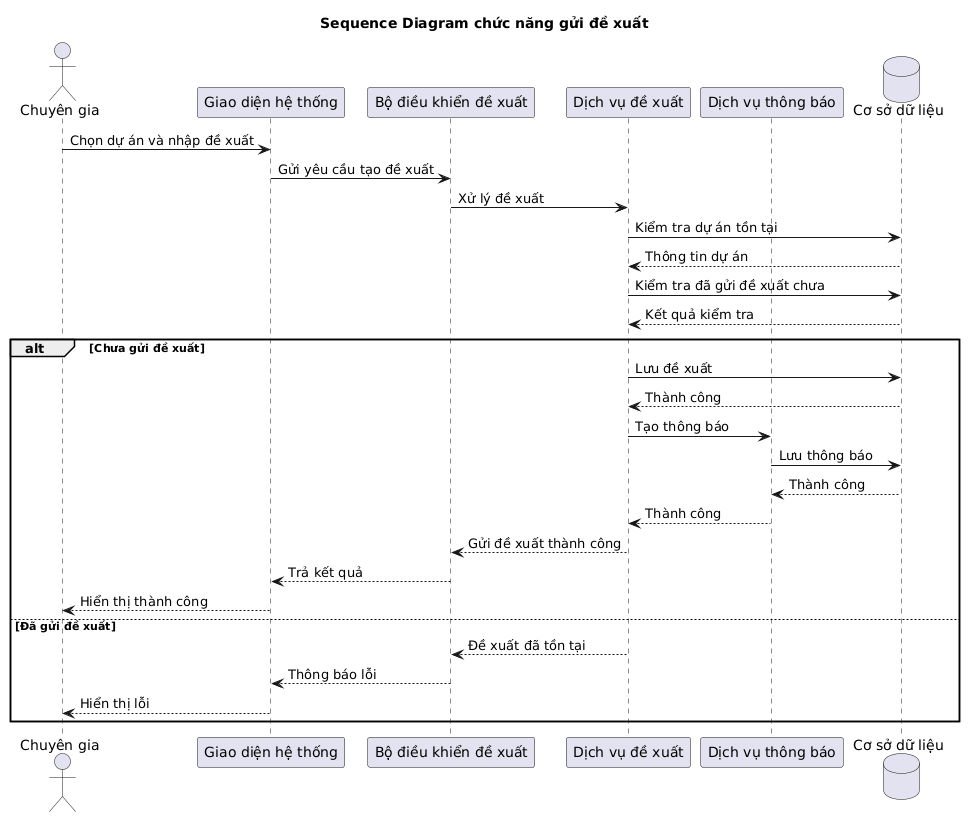
\includegraphics[width=\textwidth]{figures/sequence3.png}
\caption{Sequence Diagram chức năng chuyên gia gửi đề xuất}
\label{fig:sequence_send_proposal}
\end{figure}

Sơ đồ thể hiện kỹ thuật bẫy lỗi và chặn xử lý (Exception Handling) tại tầng nghiệp vụ. Hệ thống thực hiện các lệnh truy vấn kiểm tra điều kiện ràng buộc trước khi cho phép ghi dữ liệu đề xuất mới vào cơ sở dữ liệu.

\subsection{Sequence Diagram chức năng thuê chuyên gia}
Mô tả dòng chảy thông điệp phức tạp của tác vụ thay đổi trạng thái đồng loạt nhiều thực thể trong hệ thống.

\begin{figure}[H]
\centering
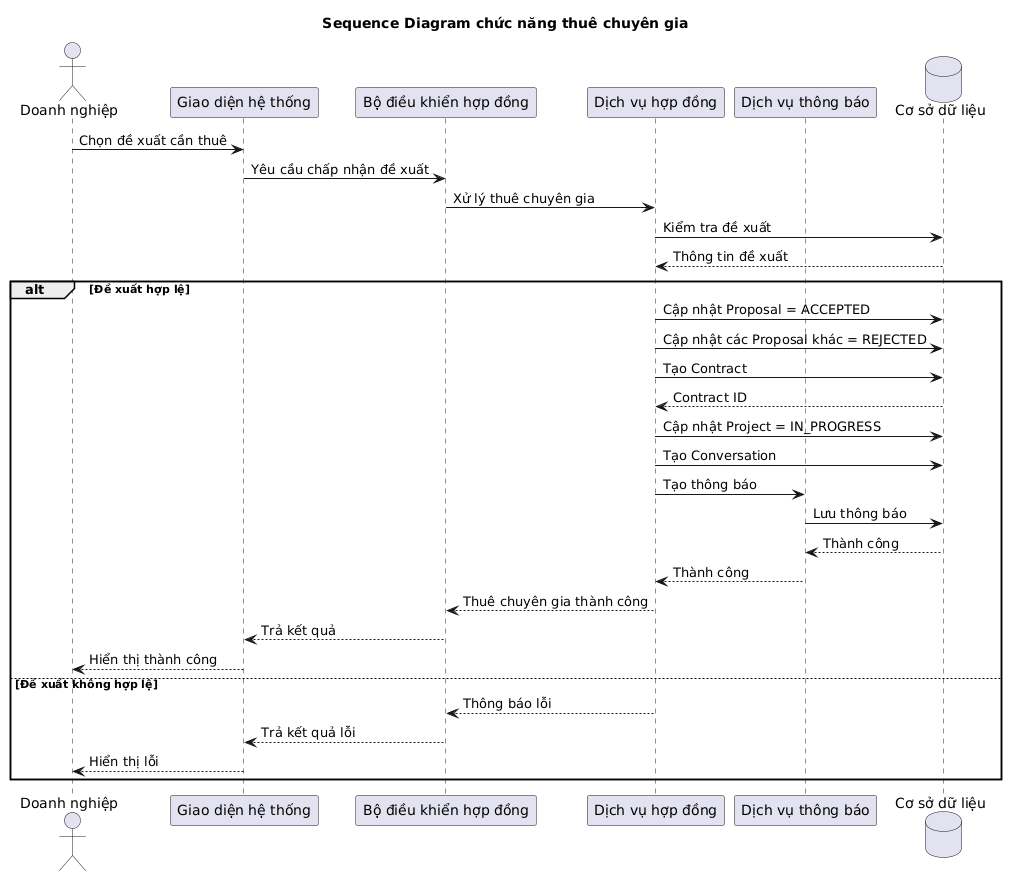
\includegraphics[width=\textwidth]{figures/sequence4.png}
\caption{Sequence Diagram chức năng phê duyệt và thuê chuyên gia}
\label{fig:sequence_hire_expert}
\end{figure}

Biểu đồ chỉ rõ tính liên kết chặt chẽ giữa các thành phần Controller, Service và Repository. Chuỗi hành động cập nhật trạng thái đề xuất, khởi tạo hợp đồng, đổi trạng thái dự án sang \texttt{IN\_PROGRESS} được thực thi tuần tự và đồng bộ.

\subsection{Sequence Diagram chức năng thanh toán}
Trình tự tương tác kết nối phân hệ tài chính nội bộ với cổng thanh toán điện tử trung gian bên thứ ba.

\begin{figure}[H]
\centering
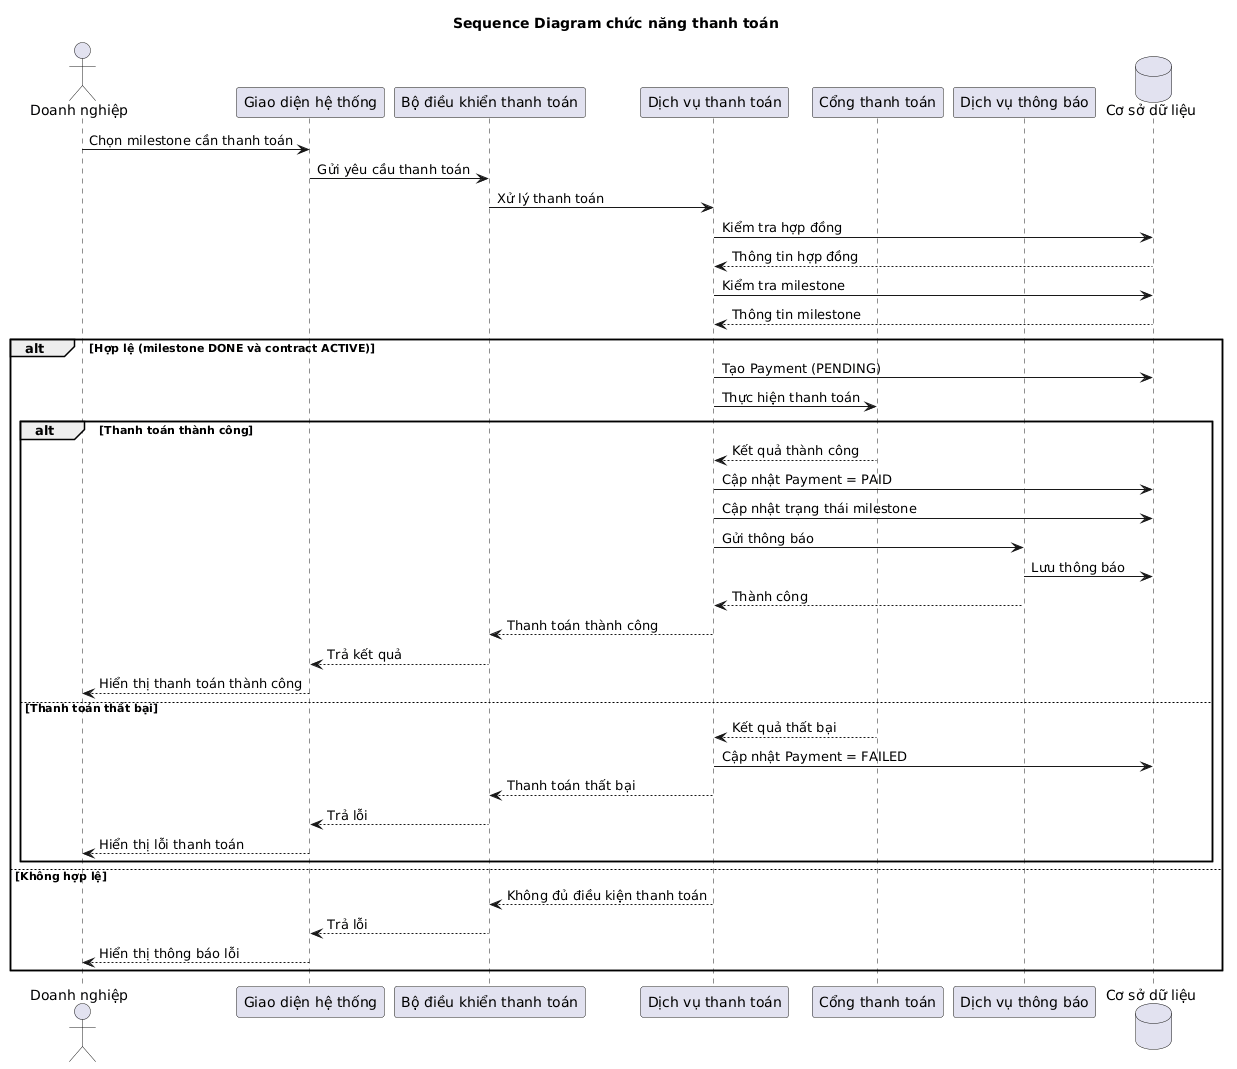
\includegraphics[width=\textwidth]{figures/sequence5.png}
\caption{Sequence Diagram chức năng thanh toán cột mốc công việc}
\label{fig:sequence_payment}
\end{figure}

Sơ đồ phân định rõ luồng xử lý bất đồng bộ khi đợi phản hồi kết quả giao dịch từ Cổng thanh toán ngoại vi (Payment Gateway). Bản ghi giao dịch được chuyển đổi trạng thái từ \texttt{PENDING} sang \texttt{PAID} hoặc \texttt{FAILED} dựa trên gói tin bảo mật trả về.

\subsection{Sequence Diagram chức năng đánh giá dự án}
Mô tả chi tiết luồng xử lý ghi nhận đánh giá và kích hoạt hàm cập nhật điểm tín nhiệm tự động.

\begin{figure}[H]
\centering
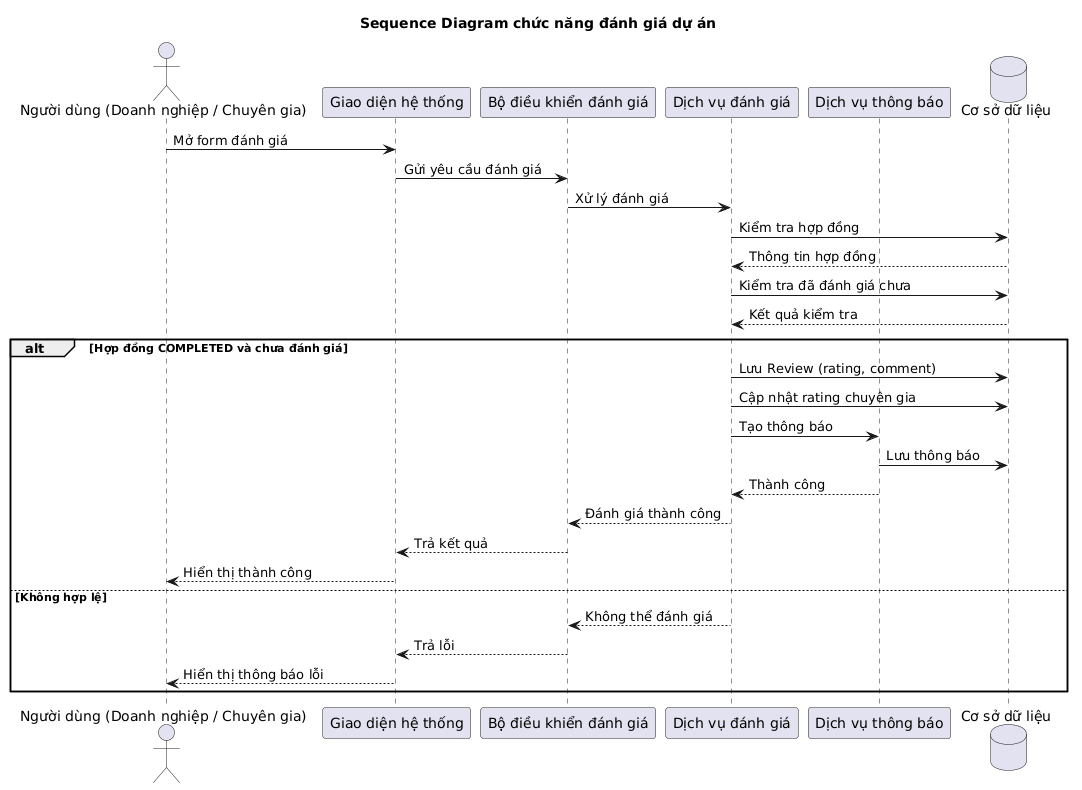
\includegraphics[width=\textwidth]{figures/sequence6.png}
\caption{Sequence Diagram chức năng đánh giá sau dự án}
\label{fig:sequence_review}
\end{figure}

Tiến trình tương tác tuần tự minh họa bước xử lý dữ liệu kép: vừa chèn bản ghi mới vào bảng \texttt{Reviews}, vừa gọi hàm tính toán cập nhật lại thuộc tính \texttt{rating} tích lũy của đối tượng nhận đánh giá tại bảng tương ứng.

\section{Biểu đồ lớp (Class Diagram)}

Class Diagram mô tả cấu trúc tĩnh, các thuộc tính định danh, các phương thức xử lý và mối liên kết logic giữa các thực thể mã nguồn của hệ thống AIConnect của hệ thống.

\begin{figure}[H]
\centering
\includegraphics[width=\textwidth]{figures/Class.png}
\caption{Biểu đồ lớp (Class Diagram) hệ thống AIConnect}
\label{fig:class_diagram}
\end{figure}

Kiến trúc lớp thể hiện rõ mô hình thiết kế hướng đối tượng:
\begin{itemize}
    \item Lớp \texttt{User} đóng vai trò là lớp cơ sở chứa các thông tin định danh cốt lõi. \texttt{Enterprise} và \texttt{Expert} liên kết chuyên biệt hóa nhằm mở rộng các thuộc tính nghiệp vụ đặc thù.
    \item Lớp \texttt{Project} đóng vai trò trung tâm liên kết với lớp danh mục \texttt{Category} và quản lý danh sách các đề xuất ứng tuyển \texttt{Proposal}.
    \item Quy trình làm việc và tài chính được quản lý chặt chẽ thông qua mối quan hệ ràng buộc giữa \texttt{Contract}, \texttt{Milestone} và \texttt{Payment}.
\end{itemize}

\section{Biểu đồ ERD}

Entity Relationship Diagram (ERD) cụ thể hóa mô hình dữ liệu quan hệ, định hình cấu trúc các bảng và các ràng buộc toàn vẹn khóa chính (PK), khóa ngoại (FK) trong cơ sở dữ liệu PostgreSQL.

\begin{figure}[H]
\centering

\includegraphics[width=\textwidth]{figures/ERD.png}
\caption{Sơ đồ thực thể quan hệ (ERD) hệ thống AIConnect}
\label{fig:erd_diagram}
\end{figure}

Sơ đồ ERD ánh xạ toàn bộ các thực thể tĩnh từ mô hình lớp thành cấu trúc lưu trữ vật lý. Mối quan hệ nhiều - nhiều giữa chuyên gia và kỹ năng được giải quyết triệt để thông qua bảng trung gian \texttt{ExpertSkills}. Các thực thể động phát sinh trong quá trình vận hành như \texttt{Messages}, \texttt{Notifications} và \texttt{Reviews} đều được thiết lập khóa ngoại liên kết trực tiếp với các định danh người dùng và hợp đồng, đảm bảo tính tra cứu và toàn vẹn dữ liệu ở mức tối đa.

\section{Kết luận chương}

Chương này đã trình bày quá trình khảo sát và phân tích yêu cầu của hệ thống \textbf{AITasker – AI Marketplace Platform for AI Automation Services}. Thông qua việc phân tích bài toán thực tế, chương đã làm rõ bối cảnh, thực trạng, nhu cầu của người dùng cũng như các mục tiêu mà hệ thống cần đáp ứng.
Trên cơ sở đó, tài liệu đặc tả yêu cầu phần mềm (Software Requirement Specification -- SRS) đã được xây dựng, bao gồm việc xác định các tác nhân tham gia, các yêu cầu chức năng và phi chức năng của hệ thống. Đồng thời, các chức năng chính như quản lý người dùng, quản lý dự án AI, gửi báo giá, trao đổi giữa doanh nghiệp và chuyên gia, theo dõi tiến độ, đánh giá và quản trị hệ thống đã được phân tích một cách chi tiết.
Bên cạnh việc đặc tả yêu cầu, chương cũng xây dựng các mô hình UML gồm Use Case Diagram, Activity Diagram, Sequence Diagram, Class Diagram và Entity Relationship Diagram (ERD). Các mô hình này mô tả trực quan quy trình nghiệp vụ, luồng xử lý và mối quan hệ giữa các thành phần trong hệ thống, góp phần bảo đảm tính nhất quán trong quá trình phân tích và thiết kế.
Những kết quả đạt được trong chương là cơ sở quan trọng cho việc thiết kế kiến trúc hệ thống, cơ sở dữ liệu và triển khai các chức năng của nền tảng \textbf{AITasker} ở các chương tiếp theo. Đồng thời, các yêu cầu được xác định trong chương này cũng là căn cứ để kiểm thử và đánh giá mức độ hoàn thiện của hệ thống sau khi xây dựng.
\chapter{Thiết kế hệ thống}

\section{Giới thiệu chương}

Sau khi hoàn thành quá trình phân tích yêu cầu hệ thống ở Chương 2, chương này trình bày thiết kế chi tiết của hệ thống AITasker. Nội dung bao gồm thiết kế kiến trúc tổng thể, thiết kế cơ sở dữ liệu, thiết kế API và thiết kế giao diện người dùng. Các nội dung được xây dựng nhằm đảm bảo hệ thống đáp ứng đầy đủ các yêu cầu chức năng và phi chức năng đã đề ra, đồng thời tạo nền tảng cho quá trình triển khai và kiểm thử ở các chương tiếp theo.

%====================================================

\section{Kiến trúc tổng thể hệ thống}

Hệ thống AITasker được xây dựng theo mô hình kiến trúc ba lớp (Three-Tier Architecture) bao gồm lớp giao diện, lớp xử lý nghiệp vụ và lớp dữ liệu.

Mô hình này giúp tách biệt các thành phần chức năng của hệ thống, tăng khả năng mở rộng, bảo trì và nâng cấp trong tương lai.

Các thành phần chính của hệ thống bao gồm:

\begin{itemize}
\item \textbf{Presentation Layer (Frontend):} Được xây dựng bằng ReactJS, cung cấp giao diện tương tác cho người dùng bao gồm doanh nghiệp, chuyên gia và quản trị viên.
\item \textbf{Business Layer (Backend):} Được phát triển bằng FastAPI, cung cấp các RESTful API xử lý nghiệp vụ của hệ thống.
\item \textbf{Data Layer (Database):} Sử dụng PostgreSQL để lưu trữ dữ liệu của hệ thống.
\item \textbf{Cloud Infrastructure:} Hệ thống được triển khai trên nền tảng Azure Cloud nhằm đảm bảo khả năng mở rộng và tính sẵn sàng cao.
\item \textbf{Storage Service:} Azure Blob Storage được sử dụng để lưu trữ hình ảnh hồ sơ, tệp đính kèm và tài liệu dự án.
\end{itemize}

\begin{figure}[H]
\centering
\includegraphics[width=\textwidth]{figures/architecture.png}
\caption{Kiến trúc tổng thể hệ thống AITasker}
\label{fig:architecture}
\end{figure}

%====================================================

\section{Thiết kế cơ sở dữ liệu}

\subsection{Tổng quan cơ sở dữ liệu}

Hệ thống sử dụng PostgreSQL làm hệ quản trị cơ sở dữ liệu quan hệ. Cơ sở dữ liệu được thiết kế dựa trên mô hình Entity Relationship Diagram (ERD) nhằm đảm bảo tính toàn vẹn dữ liệu và khả năng mở rộng.

Các bảng dữ liệu được chuẩn hóa nhằm giảm thiểu sự dư thừa và đảm bảo tính nhất quán của dữ liệu.

\subsection{Các thực thể chính}

\begin{table}[H]
\centering
\caption{Danh sách các thực thể chính}
\begin{tabular}{|p{4cm}|p{9cm}|}
\hline
\textbf{Thực thể} & \textbf{Mô tả} \\
\hline
Users & Quản lý thông tin tài khoản người dùng. \\
\hline
Enterprises & Quản lý thông tin doanh nghiệp. \\
\hline
Experts & Quản lý hồ sơ chuyên gia. \\
\hline
Skills & Danh sách kỹ năng chuyên môn. \\
\hline
Expert\_Skills & Liên kết kỹ năng với chuyên gia. \\
\hline
Categories & Danh mục dự án. \\
\hline
Projects & Thông tin dự án được đăng tải. \\
\hline
Project\_Files & Tệp đính kèm của dự án. \\
\hline
Proposals & Đề xuất của chuyên gia gửi cho dự án. \\
\hline
Contracts & Hợp đồng giữa doanh nghiệp và chuyên gia. \\
\hline
Milestones & Các giai đoạn thực hiện hợp đồng. \\
\hline
Payments & Thông tin thanh toán. \\
\hline
Conversations & Cuộc trò chuyện giữa các bên. \\
\hline
Messages & Tin nhắn trong cuộc trò chuyện. \\
\hline
Reviews & Đánh giá sau khi hoàn thành dự án. \\
\hline
Notifications & Thông báo hệ thống. \\
\hline
\end{tabular}
\end{table}

\subsection{Biểu đồ ERD}

\begin{figure}[H]
\centering

\includegraphics[width=\textwidth]{figures/ERD.png}
\caption{Biểu đồ thực thể liên kết (ERD)}
\label{fig:erd}
\end{figure}

%====================================================

\section{Thiết kế API}

Hệ thống sử dụng kiến trúc RESTful API để trao đổi dữ liệu giữa Frontend và Backend.

Các API được phân chia theo từng nhóm chức năng nhằm thuận tiện cho việc phát triển và bảo trì hệ thống.

\subsection{API xác thực}

\begin{table}[H]
\centering
\caption{Nhóm API xác thực}
\begin{tabular}{|c|p{6cm}|p{5cm}|}
\hline
Method & Endpoint & Chức năng \\
\hline
POST & /auth/register & Đăng ký tài khoản \\
\hline
POST & /auth/login & Đăng nhập hệ thống \\
\hline
GET & /auth/profile & Lấy thông tin người dùng \\
\hline
PUT & /auth/profile & Cập nhật hồ sơ cá nhân \\
\hline
\end{tabular}
\end{table}

\subsection{API dự án}

\begin{table}[H]
\centering
\caption{Nhóm API quản lý dự án}
\begin{tabular}{|c|p{6cm}|p{5cm}|}
\hline
Method & Endpoint & Chức năng \\
\hline
GET & /projects & Danh sách dự án \\
\hline
POST & /projects & Tạo dự án mới \\
\hline
GET & /projects/\{id\} & Chi tiết dự án \\
\hline
PUT & /projects/\{id\} & Cập nhật dự án \\
\hline
DELETE & /projects/\{id\} & Xóa dự án \\
\hline
\end{tabular}
\end{table}

\subsection{API đề xuất}

\begin{table}[H]
\centering
\caption{Nhóm API quản lý đề xuất}
\begin{tabular}{|c|p{6cm}|p{5cm}|}
\hline
Method & Endpoint & Chức năng \\
\hline
POST & /proposals & Gửi đề xuất \\
\hline
GET & /proposals & Danh sách đề xuất \\
\hline
PUT & /proposals/\{id\} & Cập nhật trạng thái đề xuất \\
\hline
\end{tabular}
\end{table}

\subsection{API hợp đồng và thanh toán}

\begin{table}[H]
\centering
\caption{Nhóm API hợp đồng và thanh toán}
\begin{tabular}{|c|p{6cm}|p{5cm}|}
\hline
Method & Endpoint & Chức năng \\
\hline
POST & /contracts & Tạo hợp đồng \\
\hline
GET & /contracts & Danh sách hợp đồng \\
\hline
POST & /payments & Thanh toán hợp đồng \\
\hline
GET & /payments & Danh sách giao dịch \\
\hline
\end{tabular}
\end{table}

%====================================================

\section{Thiết kế giao diện người dùng}

Giao diện người dùng được xây dựng theo mô hình Single Page Application (SPA) sử dụng ReactJS nhằm nâng cao trải nghiệm người dùng và giảm thời gian tải trang.

Các màn hình chính của hệ thống bao gồm:

\begin{itemize}
\item Trang chủ.
\item Trang đăng ký tài khoản.
\item Trang đăng nhập.
\item Trang hồ sơ doanh nghiệp.
\item Trang hồ sơ chuyên gia.
\item Trang danh sách dự án.
\item Trang chi tiết dự án.
\item Trang gửi đề xuất.
\item Trang quản lý hợp đồng.
\item Trang thanh toán.
\item Trang đánh giá.
\item Trang thông báo.
\item Trang quản trị hệ thống.
\end{itemize}

%====================================================

\section{Thiết kế bảo mật hệ thống}

Để đảm bảo an toàn dữ liệu và bảo mật thông tin người dùng, hệ thống áp dụng các cơ chế bảo mật sau:

\begin{itemize}
\item Xác thực người dùng bằng JWT (JSON Web Token).
\item Mã hóa mật khẩu bằng BCrypt.
\item Phân quyền theo vai trò (Role-Based Access Control).
\item Sử dụng giao thức HTTPS khi truyền dữ liệu.
\item Kiểm tra dữ liệu đầu vào nhằm ngăn chặn SQL Injection và XSS.
\item Giới hạn quyền truy cập đối với các API quan trọng.
\end{itemize}

%====================================================

\section{Kết luận chương}

Chương này đã trình bày thiết kế tổng thể của hệ thống AITasker bao gồm kiến trúc hệ thống, thiết kế cơ sở dữ liệu, thiết kế API, giao diện người dùng và các cơ chế bảo mật. Những nội dung này là cơ sở để triển khai hệ thống thực tế và thực hiện kiểm thử trong các chương tiếp theo.
\chapter{Yêu cầu phi chức năng}

\section{Giới thiệu}

Bên cạnh các yêu cầu chức năng, hệ thống AITasker cần đáp ứng các yêu cầu phi
chức năng nhằm đảm bảo chất lượng phần mềm, hiệu năng, độ tin cậy, tính bảo
mật và khả năng mở rộng. Các yêu cầu này đóng vai trò quan trọng trong việc
đánh giá mức độ hoàn thiện của hệ thống sau khi triển khai.

Các yêu cầu phi chức năng được xây dựng dựa trên đặc điểm của hệ thống kết nối
doanh nghiệp và chuyên gia AI, đồng thời phù hợp với kiến trúc sử dụng ReactJS,
FastAPI, PostgreSQL và các dịch vụ AI tích hợp.

%====================================================

\section{Yêu cầu về hiệu năng}

Hệ thống phải đáp ứng các yêu cầu hiệu năng sau:

\begin{itemize}

\item Thời gian phản hồi trung bình của các API không vượt quá 2 giây.

\item Chức năng đăng nhập hoàn thành trong thời gian không quá 3 giây.

\item Chức năng tạo dự án hoàn thành trong thời gian không quá 5 giây.

\item Chức năng gửi đề xuất hoàn thành trong thời gian không quá 3 giây.

\item Chức năng thanh toán Milestone hoàn thành trong thời gian không quá 5 giây.

\item Dashboard hiển thị dữ liệu trong thời gian không quá 5 giây.

\item Hệ thống hỗ trợ tối thiểu 500 người dùng hoạt động đồng thời.

\item Hệ thống có khả năng xử lý tối thiểu 100 yêu cầu mỗi giây.

\item Truy vấn cơ sở dữ liệu thông thường không vượt quá 1 giây.

\end{itemize}

%====================================================

\section{Yêu cầu về bảo mật}

Do hệ thống quản lý tài khoản, hợp đồng và thanh toán nên các yêu cầu bảo mật
được đặt ở mức cao.

\begin{itemize}

\item Người dùng phải được xác thực bằng JWT.

\item Mật khẩu được mã hóa bằng BCrypt trước khi lưu vào cơ sở dữ liệu.

\item Không lưu mật khẩu dưới dạng văn bản thuần.

\item Token phải có thời gian hết hạn.

\item Chỉ người dùng đã đăng nhập mới được truy cập các API nghiệp vụ.

\item Mỗi API phải kiểm tra quyền truy cập theo vai trò.

\item Chỉ Enterprise được phép tạo Project.

\item Chỉ Expert được phép gửi Proposal.

\item Chỉ Administrator được phép quản trị hệ thống.

\item Dữ liệu đầu vào phải được kiểm tra để hạn chế SQL Injection.

\item Dữ liệu đầu vào phải được kiểm tra nhằm hạn chế Cross Site Scripting (XSS).

\item Hệ thống hỗ trợ truyền dữ liệu thông qua HTTPS khi triển khai thực tế.

\end{itemize}

%====================================================

\section{Yêu cầu về độ tin cậy}

Hệ thống cần đảm bảo:

\begin{itemize}

\item Không làm mất dữ liệu khi xảy ra lỗi.

\item Mọi thao tác ghi dữ liệu được thực hiện bằng Transaction.

\item Dữ liệu luôn đảm bảo tính toàn vẹn.

\item Có khả năng phục hồi sau khi xảy ra sự cố.

\item Không tạo dữ liệu trùng lặp.

\item Ghi nhận nhật ký lỗi phục vụ bảo trì.

\end{itemize}

%====================================================

\section{Yêu cầu về tính sẵn sàng}

Hệ thống phải đáp ứng:

\begin{itemize}

\item Hoạt động liên tục 24 giờ mỗi ngày.

\item Thời gian sẵn sàng tối thiểu đạt 99\%.

\item Có khả năng khởi động lại sau khi máy chủ gặp sự cố.

\item Không làm gián đoạn các giao dịch đang xử lý.

\item Người dùng có thể truy cập hệ thống mọi lúc thông qua trình duyệt Web.

\end{itemize}

%====================================================

\section{Yêu cầu về khả năng mở rộng}

Hệ thống phải hỗ trợ:

\begin{itemize}

\item Gia tăng số lượng người dùng.

\item Gia tăng số lượng doanh nghiệp.

\item Gia tăng số lượng chuyên gia AI.

\item Gia tăng số lượng dự án.

\item Gia tăng số lượng hợp đồng.

\item Mở rộng cơ sở dữ liệu mà không ảnh hưởng tới hệ thống.

\item Dễ dàng tích hợp thêm các dịch vụ AI mới.

\end{itemize}

%====================================================

\section{Yêu cầu về khả năng sử dụng}

Hệ thống phải đảm bảo:

\begin{itemize}

\item Giao diện trực quan.

\item Dễ sử dụng đối với người mới.

\item Thiết kế Responsive.

\item Hỗ trợ nhiều trình duyệt.

\item Thông báo lỗi rõ ràng.

\item Điều hướng đơn giản.

\item Tìm kiếm nhanh các dự án và chuyên gia.

\item Thời gian học sử dụng hệ thống ngắn.

\end{itemize}

%====================================================

\section{Yêu cầu về khả năng bảo trì}

Để thuận tiện trong việc nâng cấp hệ thống, phần mềm phải đáp ứng:

\begin{itemize}

\item Áp dụng kiến trúc nhiều tầng.

\item Tuân thủ RESTful API.

\item Tách biệt Frontend và Backend.

\item Sử dụng SQLAlchemy ORM.

\item Có cấu trúc thư mục rõ ràng.

\item Có tài liệu API.

\item Có Logging.

\item Có Exception Handling.

\item Dễ dàng bổ sung module mới.

\end{itemize}

%====================================================

\section{Yêu cầu về khả năng tương thích}

Hệ thống hỗ trợ:

\begin{itemize}

\item Google Chrome.

\item Microsoft Edge.

\item Mozilla Firefox.

\item Windows.

\item Linux.

\item macOS.

\item PostgreSQL.

\item Python 3.12.

\item NodeJS.

\end{itemize}

%====================================================

\section{Yêu cầu về sao lưu và phục hồi}

Hệ thống cần hỗ trợ:

\begin{itemize}

\item Sao lưu dữ liệu định kỳ.

\item Khôi phục dữ liệu khi xảy ra sự cố.

\item Lưu nhật ký hệ thống.

\item Theo dõi lịch sử đăng nhập.

\item Theo dõi lịch sử thay đổi dữ liệu.

\item Khôi phục cơ sở dữ liệu từ bản sao lưu.

\end{itemize}

%====================================================

\section{Yêu cầu về tích hợp}

Hệ thống hỗ trợ tích hợp với:

\begin{itemize}

\item Google Gemini API.

\item Email Service.

\item JWT Authentication.

\item PostgreSQL.

\item Azure Cloud Storage.

\item RESTful API.

\end{itemize}

%====================================================

\section{Ràng buộc kỹ thuật}

Bảng~\ref{tab:technology} trình bày các công nghệ chính được sử dụng trong hệ
thống.

\begin{table}[H]
\centering
\caption{Các công nghệ sử dụng trong hệ thống}
\label{tab:technology}

\begin{tabular}{|p{6cm}|p{8cm}|}
\hline
\textbf{Thành phần} & \textbf{Công nghệ} \\ \hline

Frontend & ReactJS \\ \hline

Backend & FastAPI \\ \hline

Ngôn ngữ lập trình & Python 3.12 \\ \hline

Cơ sở dữ liệu & PostgreSQL \\ \hline

ORM & SQLAlchemy \\ \hline

Authentication & JWT \\ \hline

Password Hashing & BCrypt \\ \hline

AI Platform & Google Gemini API \\ \hline

Cloud Deployment & Microsoft Azure \\ \hline

API Architecture & RESTful API \\ \hline

\end{tabular}

\end{table}

%====================================================

\section{Tiêu chí chấp nhận hệ thống}

Hệ thống được xem là đáp ứng yêu cầu khi thỏa mãn các điều kiện sau:

\begin{enumerate}

\item Người dùng có thể đăng ký và đăng nhập thành công.

\item Enterprise có thể tạo Project.

\item Expert có thể gửi Proposal.

\item Enterprise có thể chấp nhận Proposal.

\item Contract được tạo đúng quy trình.

\item Milestone được quản lý đúng trạng thái.

\item Thanh toán được thực hiện thành công.

\item Người dùng có thể đánh giá sau khi hợp đồng hoàn thành.

\item Dashboard hiển thị đúng dữ liệu.

\item JWT xác thực chính xác.

\item Phân quyền theo Role hoạt động đúng.

\item Hệ thống vận hành ổn định trên các trình duyệt được hỗ trợ.

\end{enumerate}

%====================================================

\section{Kết luận}

Các yêu cầu phi chức năng là cơ sở để đánh giá chất lượng của hệ thống
AITasker sau khi triển khai. Việc đáp ứng đầy đủ các yêu cầu này sẽ giúp hệ
thống hoạt động ổn định, bảo mật, có khả năng mở rộng và đáp ứng nhu cầu sử
dụng của doanh nghiệp cũng như chuyên gia AI trong thực tế.
\chapter{Thiết kế hệ thống}

\section{Giới thiệu}

Sau khi hoàn thành quá trình phân tích yêu cầu, hệ thống AITasker được thiết kế
nhằm đảm bảo đáp ứng đầy đủ các yêu cầu chức năng và phi chức năng. Chương này
trình bày kiến trúc tổng thể, thiết kế các thành phần chính, mô hình lớp và cơ
sở dữ liệu của hệ thống.

%==============================================================

\section{Kiến trúc tổng thể}

AITasker được xây dựng theo mô hình Client--Server kết hợp kiến trúc nhiều tầng
(Multi-tier Architecture). Hệ thống gồm ba thành phần chính:

\begin{itemize}
\item Frontend: ReactJS.
\item Backend: FastAPI.
\item Database: PostgreSQL.
\end{itemize}

Ngoài ra, hệ thống còn tích hợp Google Gemini API để hỗ trợ các chức năng AI
như gợi ý mô tả dự án và chatbot hỗ trợ người dùng.

\begin{figure}[htbp]
\centering
\includegraphics[
width=\textwidth,
height=0.75\textheight,
keepaspectratio
]{architecture.png}
\caption{Kiến trúc tổng thể của hệ thống}
\label{fig:architecture}
\end{figure}

Frontend gửi yêu cầu đến Backend thông qua RESTful API. Backend xử lý nghiệp vụ,
thực hiện xác thực người dùng, thao tác với cơ sở dữ liệu và trả kết quả về giao
diện người dùng.

%==============================================================

\section{Thiết kế các thành phần}

Hệ thống được chia thành các module độc lập nhằm tăng khả năng mở rộng và bảo trì.

Các module chính gồm:

\begin{itemize}

\item Authentication

\item User Management

\item Enterprise

\item Expert

\item Project

\item Proposal

\item Contract

\item Payment

\item Review

\item Notification

\item Dashboard

\item AI Assistant

\end{itemize}

Mỗi module đảm nhiệm một nhóm chức năng riêng và giao tiếp với nhau thông qua
Service Layer.

%==============================================================

\section{Thiết kế lớp}

Hệ thống được xây dựng theo mô hình hướng đối tượng. Các lớp chính đại diện cho
các thực thể trong hệ thống như User, Enterprise, Expert, Project, Proposal,
Contract và Review.

\begin{figure}[htbp]
\centering
\includegraphics[
width=\textwidth,
height=0.80\textheight,
keepaspectratio
]{Class.png}
\caption{Biểu đồ lớp của hệ thống}
\label{fig:class}
\end{figure}

Biểu đồ lớp mô tả thuộc tính, phương thức và mối quan hệ giữa các đối tượng,
giúp việc phát triển và bảo trì hệ thống trở nên thuận lợi hơn.

%==============================================================

\section{Thiết kế cơ sở dữ liệu}

AITasker sử dụng PostgreSQL làm hệ quản trị cơ sở dữ liệu. SQLAlchemy ORM được
sử dụng để ánh xạ giữa các lớp trong chương trình và các bảng trong cơ sở dữ liệu.

Các bảng chính của hệ thống gồm:

\begin{itemize}

\item Users

\item Roles

\item Enterprises

\item Experts

\item Categories

\item Projects

\item Proposals

\item Contracts

\item Reviews

\item Notifications

\end{itemize}

\begin{figure}[htbp]
\centering

\includegraphics[
width=\textwidth,
height=0.80\textheight,
keepaspectratio
]{ERD.png}
\caption{Entity Relationship Diagram của hệ thống}
\label{fig:erd}
\end{figure}

ERD mô tả các thực thể, khóa chính, khóa ngoại và các mối quan hệ giữa các bảng,
đảm bảo dữ liệu được lưu trữ nhất quán và hạn chế dư thừa.

%==============================================================

\section{Thiết kế API và bảo mật}

Hệ thống sử dụng kiến trúc RESTful API để trao đổi dữ liệu giữa Frontend và
Backend. Dữ liệu được truyền dưới định dạng JSON.

Cơ chế bảo mật của hệ thống gồm:

\begin{itemize}

\item Xác thực bằng JWT.

\item Phân quyền theo vai trò (Administrator, Enterprise, Expert).

\item Mật khẩu được mã hóa bằng BCrypt.

\item Kiểm tra quyền truy cập tại các API.

\end{itemize}

Việc áp dụng JWT và phân quyền theo vai trò giúp đảm bảo an toàn và bảo mật
cho toàn bộ hệ thống.

%==============================================================

\section{Thiết kế tích hợp AI}

Hệ thống tích hợp Google Gemini API nhằm hỗ trợ người dùng trong quá trình sử
dụng hệ thống.

Các chức năng AI bao gồm:

\begin{itemize}

\item AI Job Assistant.

\item AI Chatbot.

\item Gợi ý mô tả dự án.

\item Hỗ trợ xây dựng yêu cầu dự án.

\end{itemize}

Việc tích hợp AI giúp nâng cao trải nghiệm người dùng và tăng hiệu quả trong
quá trình kết nối giữa doanh nghiệp và chuyên gia AI.

%==============================================================

\section{Kết luận}

Chương này đã trình bày thiết kế tổng thể của hệ thống AITasker, bao gồm kiến
trúc hệ thống, các module chức năng, biểu đồ lớp, mô hình cơ sở dữ liệu và cơ
chế bảo mật. Đây là cơ sở để triển khai hệ thống và kiểm thử trong các chương
tiếp theo.
\chapter{Cài đặt và triển khai hệ thống}

\section{Giới thiệu}

Sau khi hoàn thành giai đoạn phân tích yêu cầu và thiết kế hệ thống, bước tiếp
theo là hiện thực hóa hệ thống AITasker thông qua việc xây dựng các thành phần
phần mềm và triển khai trên môi trường thực tế.

Chương này trình bày môi trường phát triển, công nghệ sử dụng, cấu trúc mã
nguồn, quy trình triển khai cũng như các thành phần chính của hệ thống.

%============================================================

\section{Môi trường phát triển}

Hệ thống được phát triển trên môi trường Windows với các công cụ được trình bày
trong Bảng~\ref{tab:development_environment}.

\begin{table}[H]
\centering
\caption{Môi trường phát triển hệ thống}
\label{tab:development_environment}

\begin{tabular}{|p{6cm}|p{8cm}|}
\hline
\textbf{Thành phần} & \textbf{Phiên bản} \\ \hline

Hệ điều hành & Windows 11 \\ \hline

Python & 3.12 \\ \hline

NodeJS & 20.x \\ \hline

ReactJS & 18.x \\ \hline

FastAPI & 0.115.x \\ \hline

PostgreSQL & 16.x \\ \hline

SQLAlchemy & 2.x \\ \hline

Visual Studio Code & Latest \\ \hline

Git & Latest \\ \hline

Postman & Latest \\ \hline

\end{tabular}

\end{table}

%============================================================

\section{Kiến trúc triển khai}

Hệ thống được triển khai theo mô hình Client--Server.

\begin{itemize}

\item Frontend được xây dựng bằng ReactJS.

\item Backend được xây dựng bằng FastAPI.

\item PostgreSQL lưu trữ dữ liệu.

\item SQLAlchemy ORM thực hiện ánh xạ dữ liệu.

\item JWT dùng để xác thực người dùng.

\item Google Gemini API hỗ trợ các chức năng AI.

\item Azure Cloud Storage lưu trữ tệp.

\end{itemize}

%============================================================

\section{Cấu trúc mã nguồn}

Hệ thống được chia thành hai phần chính:

\begin{itemize}

\item Frontend

\item Backend

\end{itemize}

\subsection{Frontend}

Frontend được phát triển bằng ReactJS với cấu trúc thư mục như sau:

\begin{lstlisting}
frontend/
│
├── public/
├── src/
│   ├── assets/
│   ├── components/
│   ├── pages/
│   ├── layouts/
│   ├── services/
│   ├── hooks/
│   ├── routes/
│   ├── utils/
│   └── App.jsx
└── package.json
\end{lstlisting}

\subsection{Backend}

Backend được xây dựng bằng FastAPI.

\begin{lstlisting}
backend/
│
├── src/
│   ├── config/
│   ├── models/
│   ├── schemas/
│   ├── services/
│   ├── presentation/
│   ├── middleware/
│   ├── utils/
│   ├── uploads/
│   └── app.py
│
├── migrations/
└── requirements.txt
\end{lstlisting}

%============================================================

\section{Các module đã triển khai}

Các module chính của hệ thống gồm:

\begin{itemize}

\item Authentication

\item User Management

\item Enterprise Management

\item Expert Management

\item Category Management

\item Skill Management

\item Project Management

\item Proposal Management

\item Contract Management

\item Milestone Management

\item Payment Management

\item Review Management

\item Notification Management

\item Dashboard

\item Statistics

\end{itemize}

%============================================================

\section{Cơ chế xác thực}

Hệ thống sử dụng JWT để xác thực người dùng.

Quy trình hoạt động:

\begin{enumerate}

\item Người dùng đăng nhập.

\item Backend kiểm tra thông tin.

\item Sinh JWT.

\item JWT được gửi về Frontend.

\item Frontend lưu Access Token.

\item Token được gửi kèm mỗi yêu cầu.

\item Backend xác thực Token.

\item Nếu hợp lệ, yêu cầu được xử lý.

\end{enumerate}

%============================================================

\section{Quản lý cơ sở dữ liệu}

Hệ thống sử dụng PostgreSQL kết hợp SQLAlchemy ORM.

Các bảng dữ liệu chính gồm:

\begin{itemize}

\item users

\item roles

\item permissions

\item enterprises

\item experts

\item projects

\item proposals

\item contracts

\item milestones

\item payments

\item reviews

\item notifications

\item conversations

\item messages

\item skills

\item categories

\end{itemize}

%============================================================

\section{Triển khai RESTful API}

Backend cung cấp RESTful API cho Frontend.

Các nhóm API bao gồm:

\begin{itemize}

\item Authentication API

\item User API

\item Enterprise API

\item Expert API

\item Category API

\item Skill API

\item Project API

\item Proposal API

\item Contract API

\item Milestone API

\item Payment API

\item Review API

\item Notification API

\item Dashboard API

\item Statistics API

\end{itemize}

%============================================================

\section{Quản lý tệp}

Hệ thống hỗ trợ tải lên các loại tệp:

\begin{itemize}

\item Ảnh đại diện.

\item CV.

\item Portfolio.

\item Tệp mô tả dự án.

\item Deliverable.

\end{itemize}

Các tệp được lưu trên Azure Cloud Storage hoặc thư mục Upload của hệ thống.

%============================================================

\section{Triển khai AI}

AITasker tích hợp Google Gemini API để hỗ trợ:

\begin{itemize}

\item AI Job Assistant.

\item Gợi ý nội dung Project.

\item Hỗ trợ tạo mô tả công việc.

\item Chatbot hỗ trợ người dùng.

\end{itemize}

%============================================================

\section{Triển khai hệ thống}

Quy trình triển khai gồm các bước:

\begin{enumerate}

\item Cài đặt Python.

\item Cài đặt NodeJS.

\item Cài đặt PostgreSQL.

\item Clone mã nguồn.

\item Cài đặt thư viện Backend.

\item Cài đặt thư viện Frontend.

\item Khởi tạo cơ sở dữ liệu.

\item Chạy Backend.

\item Chạy Frontend.

\item Kiểm tra hệ thống.

\end{enumerate}

%============================================================

\section{Hướng dẫn chạy hệ thống}

Khởi động Backend:

\begin{lstlisting}[language=bash]
uvicorn backend.src.app:app --reload
\end{lstlisting}

Khởi động Frontend:

\begin{lstlisting}[language=bash]
npm install
npm run dev
\end{lstlisting}

Sau khi khởi động thành công:

\begin{itemize}

\item Frontend:
\url{http://localhost:5173}

\item Backend:
\url{http://localhost:8000}

\item Swagger UI:
\url{http://localhost:8000/docs}

\end{itemize}

%============================================================

\section{Đánh giá kết quả triển khai}

Sau khi triển khai, hệ thống đạt được các kết quả sau:

\begin{itemize}

\item Đăng ký và đăng nhập hoạt động ổn định.

\item Phân quyền người dùng chính xác.

\item Doanh nghiệp có thể tạo Project.

\item Chuyên gia có thể gửi Proposal.

\item Có thể tạo Contract.

\item Quản lý Milestone hoạt động đúng.

\item Thanh toán hoạt động theo quy trình.

\item Dashboard hiển thị dữ liệu.

\item API phản hồi đúng định dạng JSON.

\item PostgreSQL lưu trữ dữ liệu ổn định.

\end{itemize}

%============================================================

\section{Kết luận}

Hệ thống AITasker đã được hiện thực thành công dựa trên kiến trúc Client--Server
với Frontend ReactJS, Backend FastAPI và cơ sở dữ liệu PostgreSQL. Các module
chính đã được triển khai theo đúng thiết kế, đáp ứng các yêu cầu chức năng và
phi chức năng đã đề ra.

Việc sử dụng các công nghệ hiện đại như SQLAlchemy ORM, JWT Authentication,
Google Gemini API và Azure Cloud Storage giúp hệ thống có khả năng mở rộng,
dễ bảo trì và sẵn sàng cho việc triển khai thực tế.
\chapter{Kiểm thử và đánh giá hệ thống}

\section{Giới thiệu}

Sau khi hoàn thành quá trình cài đặt và triển khai, hệ thống AITasker được tiến
hành kiểm thử nhằm đánh giá mức độ đáp ứng các yêu cầu chức năng và phi chức
năng đã được đặc tả. Quá trình kiểm thử giúp phát hiện các lỗi còn tồn tại,
đánh giá tính ổn định, hiệu năng và khả năng sử dụng của hệ thống trước khi đưa
vào sử dụng.

Trong phạm vi đồ án, nhóm tập trung thực hiện kiểm thử chức năng (Functional
Testing) kết hợp với kiểm thử tích hợp (Integration Testing) và kiểm thử giao
diện người dùng.

%============================================================

\section{Môi trường kiểm thử}

Quá trình kiểm thử được thực hiện trong môi trường trình bày ở
Bảng~\ref{tab:test_environment}.

\begin{table}[H]
\centering
\caption{Môi trường kiểm thử}
\label{tab:test_environment}

\begin{tabular}{|p{6cm}|p{8cm}|}
\hline
\textbf{Thành phần} & \textbf{Thông tin} \\ \hline

Hệ điều hành & Windows 11 \\ \hline

Backend & FastAPI \\ \hline

Frontend & ReactJS \\ \hline

Database & PostgreSQL \\ \hline

API Testing & Swagger UI, Postman \\ \hline

IDE & Visual Studio Code \\ \hline

Trình duyệt & Google Chrome \\ \hline

\end{tabular}

\end{table}

%============================================================

\section{Phương pháp kiểm thử}

Các phương pháp kiểm thử được áp dụng bao gồm:

\begin{itemize}

\item Kiểm thử chức năng.

\item Kiểm thử giao diện.

\item Kiểm thử tích hợp.

\item Kiểm thử API.

\item Kiểm thử phân quyền.

\item Kiểm thử dữ liệu đầu vào.

\end{itemize}

%============================================================

\section{Các chức năng được kiểm thử}

Nhóm tiến hành kiểm thử các chức năng chính của hệ thống:

\begin{enumerate}

\item Đăng ký tài khoản.

\item Đăng nhập.

\item Quản lý hồ sơ.

\item Tạo Project.

\item Cập nhật Project.

\item Gửi Proposal.

\item Chấp nhận Proposal.

\item Tạo Contract.

\item Quản lý Milestone.

\item Thanh toán.

\item Đánh giá.

\item Dashboard.

\item Notification.

\end{enumerate}

%============================================================

\section{Các trường hợp kiểm thử}

\subsection{Kiểm thử chức năng đăng ký}

\begin{table}[H]
\centering
\caption{Kiểm thử chức năng đăng ký}
\begin{tabular}{|p{2cm}|p{4cm}|p{4cm}|p{4cm}|}
\hline

\textbf{Test ID}
&
\textbf{Dữ liệu đầu vào}
&
\textbf{Kết quả mong đợi}
&
\textbf{Kết quả}
\\
\hline

TC01
&
Thông tin hợp lệ
&
Đăng ký thành công
&
Đạt
\\
\hline

TC02
&
Email đã tồn tại
&
Thông báo lỗi
&
Đạt
\\
\hline

TC03
&
Mật khẩu dưới 8 ký tự
&
Thông báo lỗi
&
Đạt
\\
\hline

\end{tabular}

\end{table}

%============================================================

\subsection{Kiểm thử chức năng đăng nhập}

\begin{table}[H]
\centering
\caption{Kiểm thử chức năng đăng nhập}

\begin{tabular}{|p{2cm}|p{4cm}|p{4cm}|p{4cm}|}

\hline

TC04
&
Email và mật khẩu đúng
&
Đăng nhập thành công
&
Đạt
\\
\hline

TC05
&
Sai mật khẩu
&
Thông báo lỗi
&
Đạt
\\
\hline

TC06
&
Email không tồn tại
&
Thông báo lỗi
&
Đạt
\\
\hline

\end{tabular}

\end{table}

%============================================================

\subsection{Kiểm thử chức năng tạo Project}

\begin{table}[H]

\centering

\caption{Kiểm thử chức năng tạo Project}

\begin{tabular}{|p{2cm}|p{4cm}|p{4cm}|p{4cm}|}

\hline

TC07
&
Thông tin hợp lệ
&
Project được tạo
&
Đạt
\\
\hline

TC08
&
Thiếu tiêu đề
&
Thông báo lỗi
&
Đạt
\\
\hline

TC09
&
Ngân sách âm
&
Thông báo lỗi
&
Đạt
\\
\hline

\end{tabular}

\end{table}

%============================================================

\subsection{Kiểm thử chức năng gửi Proposal}

\begin{table}[H]

\centering

\caption{Kiểm thử chức năng gửi Proposal}

\begin{tabular}{|p{2cm}|p{4cm}|p{4cm}|p{4cm}|}

\hline

TC10
&
Thông tin hợp lệ
&
Proposal được tạo
&
Đạt
\\
\hline

TC11
&
Đã gửi Proposal
&
Thông báo lỗi
&
Đạt
\\
\hline

\end{tabular}

\end{table}

%============================================================

\subsection{Kiểm thử chức năng thanh toán}

\begin{table}[H]

\centering

\caption{Kiểm thử chức năng thanh toán}

\begin{tabular}{|p{2cm}|p{4cm}|p{4cm}|p{4cm}|}

\hline

TC12
&
Milestone hợp lệ
&
Thanh toán thành công
&
Đạt
\\
\hline

TC13
&
Milestone chưa hoàn thành
&
Thông báo lỗi
&
Đạt
\\
\hline

\end{tabular}

\end{table}

%============================================================

\section{Kiểm thử API}

Nhóm sử dụng Swagger UI và Postman để kiểm thử các RESTful API.

Các API đã được kiểm thử gồm:

\begin{itemize}

\item Authentication API

\item User API

\item Enterprise API

\item Expert API

\item Project API

\item Proposal API

\item Contract API

\item Milestone API

\item Review API

\item Notification API

\item Dashboard API

\end{itemize}

Tất cả API đều trả về đúng định dạng JSON và mã trạng thái HTTP tương ứng.

%============================================================

\section{Kiểm thử giao diện}

Giao diện hệ thống được kiểm thử trên các trình duyệt:

\begin{itemize}

\item Google Chrome

\item Microsoft Edge

\item Mozilla Firefox

\end{itemize}

Kết quả cho thấy giao diện hiển thị đúng, bố cục hợp lý và hỗ trợ Responsive
trên các kích thước màn hình phổ biến.

%============================================================

\section{Kiểm thử phân quyền}

Các vai trò được kiểm thử gồm:

\begin{itemize}

\item Administrator

\item Enterprise

\item Expert

\end{itemize}

Kết quả kiểm thử cho thấy:

\begin{itemize}

\item Administrator có toàn quyền quản trị.

\item Enterprise chỉ được thao tác trên Project và Contract của mình.

\item Expert chỉ được gửi Proposal và thực hiện Contract.

\item Người dùng chưa đăng nhập không thể truy cập các API bảo vệ.

\end{itemize}

%============================================================

\section{Đánh giá hệ thống}

Sau quá trình kiểm thử, hệ thống đạt được các kết quả sau:

\begin{itemize}

\item Các chức năng chính hoạt động đúng yêu cầu.

\item Phân quyền hoạt động chính xác.

\item API phản hồi đúng dữ liệu.

\item JWT xác thực ổn định.

\item PostgreSQL lưu trữ dữ liệu chính xác.

\item Hệ thống vận hành ổn định.

\item Giao diện thân thiện.

\item Kiến trúc dễ mở rộng.

\end{itemize}

%============================================================

\section{Hạn chế}

Mặc dù hệ thống đã đáp ứng hầu hết các yêu cầu đặt ra, vẫn còn một số hạn chế:

\begin{itemize}

\item Chưa tích hợp cổng thanh toán thực tế.

\item Chưa triển khai AI Recommendation.

\item Chưa triển khai WebSocket cho thông báo thời gian thực.

\item Chưa có ứng dụng di động.

\item Chưa thực hiện kiểm thử tải (Load Testing) và kiểm thử hiệu năng chuyên sâu.

\end{itemize}

%============================================================

\section{Hướng phát triển}

Trong tương lai, hệ thống có thể được mở rộng theo các hướng sau:

\begin{itemize}

\item Tích hợp Stripe hoặc PayPal.

\item Tích hợp AI Recommendation System.

\item Tích hợp AI Chatbot nâng cao.

\item Triển khai Docker và Kubernetes.

\item Triển khai CI/CD.

\item Xây dựng ứng dụng Android và iOS.

\item Bổ sung hệ thống giám sát và cảnh báo.

\item Tối ưu hiệu năng cơ sở dữ liệu.

\end{itemize}

%============================================================

\section{Kết luận}

Qua quá trình kiểm thử, hệ thống AITasker đáp ứng đầy đủ các yêu cầu chức năng
và phần lớn các yêu cầu phi chức năng đã đề ra. Các chức năng chính hoạt động
ổn định, dữ liệu được quản lý chính xác và cơ chế phân quyền đảm bảo an toàn.
Mặc dù vẫn còn một số hạn chế cần tiếp tục cải thiện, hệ thống đã sẵn sàng để
phát triển và triển khai trong các giai đoạn tiếp theo.

% ==========================================================
% KẾT LUẬN VÀ HƯỚNG PHÁT TRIỂN
% ==========================================================

\chapter*{Kết luận và hướng phát triển}
\addcontentsline{toc}{chapter}{Kết luận và hướng phát triển}

\section*{Kết luận}

Đề tài \projectname{} đã xây dựng một nền tảng hỗ trợ kết nối giữa doanh
nghiệp có nhu cầu ứng dụng trí tuệ nhân tạo và các chuyên gia có năng lực
triển khai giải pháp AI.

Hệ thống được xây dựng theo kiến trúc Client--Server với Frontend sử dụng
ReactJS, Backend sử dụng FastAPI và cơ sở dữ liệu PostgreSQL. Các chức năng
chính gồm quản lý tài khoản, xác thực và phân quyền, quản lý doanh nghiệp,
quản lý chuyên gia, tạo dự án, gửi đề xuất, quản lý hợp đồng, quản lý tiến độ,
thanh toán, đánh giá, thông báo và hỗ trợ người dùng bằng trí tuệ nhân tạo.

Báo cáo đã trình bày các yêu cầu chức năng, yêu cầu phi chức năng, kiến trúc
hệ thống, mô hình dữ liệu, các sơ đồ UML, quá trình triển khai và các trường
hợp kiểm thử. Các kết quả đạt được cho thấy hệ thống có khả năng đáp ứng các
nghiệp vụ cơ bản của một nền tảng kết nối doanh nghiệp và chuyên gia AI.

\section*{Hướng phát triển}

Trong tương lai, hệ thống có thể được tiếp tục phát triển theo các hướng sau:

\begin{itemize}
    \item Hoàn thiện cơ chế ký quỹ và giải ngân tự động.
    \item Tích hợp cổng thanh toán trực tuyến thực tế.
    \item Phát triển hệ thống gợi ý chuyên gia bằng học máy.
    \item Nâng cao khả năng phân tích yêu cầu dự án bằng AI.
    \item Tích hợp thông báo thời gian thực bằng WebSocket.
    \item Hoàn thiện dịch vụ gửi email và khôi phục mật khẩu.
    \item Phát triển ứng dụng trên thiết bị di động.
    \item Triển khai hệ thống trên nền tảng điện toán đám mây.
    \item Bổ sung kiểm thử tự động và quy trình CI/CD.
    \item Nâng cao khả năng giám sát, sao lưu và bảo mật dữ liệu.
\end{itemize}

\clearpage

% ==========================================================
% TÀI LIỆU THAM KHẢO
% ==========================================================

\printbibliography[
    heading=bibintoc,
    title={Tài liệu tham khảo}
]

\clearpage

% ==========================================================
% PHỤ LỤC
% ==========================================================

\appendix

\IfFileExists{appendix/appendix_a.tex}{
    \input{appendix/appendix_a}
}{
    \chapter{Phụ lục}

    Nội dung phụ lục sẽ được bổ sung trong phiên bản hoàn thiện của báo cáo.
}

\end{document}